\documentclass[11pt,a4paper]{article}

% ============================================================
%  SEA -- Segment, Embed, and Align
%  A Deep Technical Report on the Pipeline Implemented in this
%  Workspace for Thai Sign Language (TSL) Subtitle Alignment
% ============================================================

\usepackage[a4paper,margin=2.3cm]{geometry}
\usepackage[T1]{fontenc}
\usepackage[utf8]{inputenc}

% ---------- Fonts: Palatino body + Helvetica-style sans + Inconsolata mono ----------
% A clean, professional combination using widely-available packages.
\usepackage{amsmath,amssymb,amsthm}
\usepackage{mathpazo}                   % Palatino body + matching math
\usepackage[scaled=0.95]{helvet}        % sans-serif (Helvetica) for headings
\usepackage[scaled=0.92]{inconsolata}   % monospace for code listings

\usepackage{microtype}
\usepackage{graphicx}
\usepackage{xcolor}
\usepackage{booktabs}
\usepackage{array}
\usepackage{tabularx}
\usepackage{longtable}
\usepackage{enumitem}
\usepackage{caption}
\usepackage{subcaption}
\usepackage{listings}
\usepackage[hidelinks,colorlinks=true,linkcolor=blue!50!black,
            urlcolor=blue!50!black,citecolor=blue!50!black,
            pdftitle={SEA Pipeline Report -- TSL Subtitle Alignment},
            pdfauthor={NECTEC/SEA workspace},
            bookmarksnumbered=true]{hyperref}
\usepackage{titlesec}
\usepackage{fancyhdr}
\usepackage{multirow}

% ---------- TikZ for pipeline diagrams ----------
\usepackage{tikz}
\usetikzlibrary{arrows.meta,positioning,calc,fit,shapes.geometric,shapes.misc,backgrounds,decorations.pathreplacing,patterns}

% ---------- Sans-serif captions ----------
\captionsetup{font={small,sf},labelfont={bf,sf},labelsep=period}

% ---------- Listings style ----------
\definecolor{codebg}{rgb}{0.97,0.97,0.97}
\definecolor{codekw}{rgb}{0.10,0.30,0.70}
\definecolor{codestr}{rgb}{0.55,0.10,0.10}
\definecolor{codecmt}{rgb}{0.30,0.55,0.30}

\lstdefinestyle{plainstyle}{
  basicstyle=\ttfamily\footnotesize,
  backgroundcolor=\color{codebg},
  keywordstyle=\color{codekw}\bfseries,
  stringstyle=\color{codestr},
  commentstyle=\color{codecmt}\itshape,
  frame=single,
  framerule=0.3pt,
  rulecolor=\color{black!30},
  breaklines=true,
  breakatwhitespace=false,
  columns=fullflexible,
  showstringspaces=false,
  tabsize=2,
  xleftmargin=6pt,
  xrightmargin=6pt
}
\lstset{style=plainstyle}

% ---------- TikZ block-diagram styles ----------
\definecolor{stageInput}{HTML}{F5E6D3}    % parchment for inputs
\definecolor{stageInputBd}{HTML}{B58A60}
\definecolor{stageSeg}{HTML}{FFE7B3}      % yellow for Segment
\definecolor{stageSegBd}{HTML}{C6932A}
\definecolor{stageEmb}{HTML}{D4E7F7}      % blue for Embed
\definecolor{stageEmbBd}{HTML}{2E6CB1}
\definecolor{stageAlign}{HTML}{D6EFD8}    % green for Align
\definecolor{stageAlignBd}{HTML}{3A8C46}
\definecolor{stagePost}{HTML}{F2D7E2}     % pink for post-processing
\definecolor{stagePostBd}{HTML}{B0497A}

\tikzset{
  stage/.style={
    rectangle, rounded corners=4pt, draw=black!60,
    minimum width=46mm, minimum height=10mm,
    align=center, font=\small\sffamily,
    inner sep=4pt
  },
  data/.style={
    stage, fill=stageInput, draw=stageInputBd,
    font=\footnotesize\sffamily,
    minimum width=42mm, minimum height=8mm,
    rounded corners=2pt
  },
  seg/.style ={stage, fill=stageSeg,   draw=stageSegBd},
  emb/.style ={stage, fill=stageEmb,   draw=stageEmbBd},
  ali/.style ={stage, fill=stageAlign, draw=stageAlignBd},
  post/.style={stage, fill=stagePost,  draw=stagePostBd},
  flow/.style={-{Stealth[length=2.5mm,width=2mm]}, thick, draw=black!70},
  legend/.style={font=\footnotesize\sffamily}
}

% ---------- Page style ----------
\pagestyle{fancy}
\fancyhf{}
\fancyhead[L]{\small\sffamily SEA Pipeline Report}
\fancyhead[R]{\small\sffamily TSL Subtitle Alignment}
\fancyfoot[C]{\sffamily\thepage}
\renewcommand{\headrulewidth}{0.4pt}

\titleformat{\section}{\Large\bfseries\sffamily}{\thesection}{0.7em}{}
\titleformat{\subsection}{\large\bfseries\sffamily}{\thesubsection}{0.6em}{}
\titleformat{\subsubsection}{\normalsize\bfseries\sffamily}{\thesubsubsection}{0.5em}{}

% Make `\texttt` safe inside section titles for PDF bookmarks
\pdfstringdefDisableCommands{%
  \def\texttt#1{#1}%
  \def\textbf#1{#1}%
  \def\textit#1{#1}%
  \def\emph#1{#1}%
}

% ---------- Title ----------
\title{\textbf{SEA: Segment, Embed, and Align} \\[6pt]
       \large A Deep Technical Walkthrough of the Subtitle Alignment Pipeline \\
       Applied to Thai Sign Language --- with Background from the Original Paper \\
       and Live Experimental Results from this Workspace}
\author{Generated technical report \\
        Workspace: \texttt{NECTEC/SEA}}
\date{\today}

\begin{document}
\maketitle

\begin{abstract}
\noindent
This report explains, in deep technical detail, the \emph{Segment, Embed, and
Align} (SEA) pipeline as it is implemented in this workspace and applied to a
Thai Sign Language (TSL) example video. It is organised in three layers:
\textbf{(i)} an introduction to SEA as published in the original paper
\emph{``Segment, Embed, and Align: A Universal Recipe for Aligning Subtitles to
Signing''} by Jiang et al., 2025
(\href{https://arxiv.org/abs/2512.08094}{arXiv:2512.08094}), including its
motivation, formal task definition, full algorithmic description, the four
benchmark datasets, and the SOTA results published by the authors;
\textbf{(ii)} a step-by-step technical breakdown of the pipeline as it is
actually run in this workspace---inputs, intermediate artefacts, command
lines, parameters, internal mathematics, code locations, and outputs;
\textbf{(iii)} a complete report of the experimental results obtained on a real
TSL lecture video (172 captions, 11~min 07~s) covering nine experiments
(\texttt{A}, \texttt{B1}, \texttt{B2}, \texttt{B\_MULTI}, \texttt{C\_MULTI},
\texttt{C\_MULTI\_word}, \texttt{D\_ASL}, \texttt{D\_ASL\_gloss},
\texttt{D\_ASL\_word}), including verified live numbers obtained by re-running
\texttt{evaluate\_all.py} during the writing of this report.
\end{abstract}

\tableofcontents
\clearpage

% ============================================================
\part{Background --- the SEA Paper}
% ============================================================

\section{Motivation: Why Sign-Language Subtitle Alignment?}
\label{sec:motivation}

Sign-language alignment is the task of taking written subtitles---which were
originally produced for the audio track of a programme---and shifting their
timestamps so that they coincide with the moment a signer actually performs
the corresponding signs. The original SEA paper opens with two practical
reasons this matters.

\paragraph{Parallel data for sign-language translation.} The current generation
of sign-language translation systems
\cite{muller-etal-2022-findings,muller-etal-2023-findings}
is data-hungry, and the largest broadcast corpora---most notably BOBSL
(46\,h of BBC interpreted television)---ship with subtitles that are
\emph{audio-aligned}, not \emph{sign-aligned}. Hearing interpreters who must
listen and then sign always lag the audio by 1--3\,s, so the off-the-shelf
captions are systematically misplaced. Re-aligning them is a precondition for
training translation models that learn the correct text$\leftrightarrow$sign
correspondence.

\paragraph{Accessibility and post-hoc captioning.} For deaf viewers of
user-generated YouTube content, automatic alignment of a noisy first-pass
caption file dramatically reduces the human effort needed to ship usable
subtitles. The SEA paper cites Bull et al.\ 2021's measurement that an expert
fluent in sign language takes 10--15\,h to align subtitles to one hour of
video manually; at the WMT-SLT~22 rate of \$40/hour, that is \$400--600 of
labour per programme hour. Anything that compresses this cost has direct
practical impact.

\paragraph{Why prior approaches are limited.} Two end-to-end models are the
state of the art before SEA: \emph{SAT} (Bull et al., 2021) and its successor
\emph{SAT$^{+}$} (Jang et al., 2025). Both are transformer encoders fine-tuned
on $\sim$17.7\,h of \emph{manually aligned} BSL/English data---i.e.\ they
already need the very thing one is trying to produce. They also predict at the
frame level inside a 20-second sliding window and then resolve cross-window
conflicts with dynamic time warping (DTW), which is fundamentally local.

\paragraph{The SEA proposition.} SEA is presented as a \emph{training-free,
language-universal} alternative. It assumes the existence of two pretrained
sign-language models (a segmenter and an embedder) and replaces the
trained-aligner with a global, gradient-free dynamic programme over the
\emph{whole episode}. The trade-off: a small parameter search per dataset, in
exchange for no in-domain alignment supervision and a fully modular pipeline.


\section{Formal Task and Three-Stage Pipeline}
\label{sec:formal-task}

\subsection{Inputs and outputs}
\paragraph{Given.} A continuous sign-language video and a sequence of subtitle
units $t_1, \ldots, t_n$ each with a (possibly noisy) start and end time
$\bigl(\mathrm{start}(t_i), \mathrm{end}(t_i)\bigr)$.
\paragraph{Goal.} Adjust the start/end timestamps of every $t_i$ so that they
better match the signing.

\subsection{The three modular stages}
SEA factors the problem into three plug-and-play steps; the first two are
pretrained models, the third is the new contribution.
\begin{enumerate}[leftmargin=1.5em]
  \item \textbf{Segment} the continuous video frames into individual signs
        $s_1, \ldots, s_m$ with $\bigl(\mathrm{start}(s_j), \mathrm{end}(s_j)\bigr)$.
        This is analogous to text tokenisation but without a standardised
        vocabulary.
  \item \textbf{Embed} every sign $s_j$ and every subtitle unit $t_i$ into a
        \emph{shared} latent space $\mathbb{R}^d$. Cross-modal similarity
        $\langle u_i, v_j \rangle$ then has a meaning.
  \item \textbf{Align}: choose, for every $t_i$, a \emph{contiguous} span
        $\{s_l, \ldots, s_r\}$ that minimises a global cost combining
        timing/prosodic terms and (optionally) the semantic similarity
        provided by the embeddings; rewrite $t_i$'s timestamps to the chosen
        span's boundaries.
\end{enumerate}

The paper distinguishes two algorithmic variants:
\textbf{Segment and Align} (timing-only) and \textbf{Segment, Embed, and
Align} (timing + semantics). Both use the same DP recurrence; the second adds
one extra term to the cost.

% ----------- High-level architecture diagram (paper view) -----------
\begin{figure}[h]
\centering
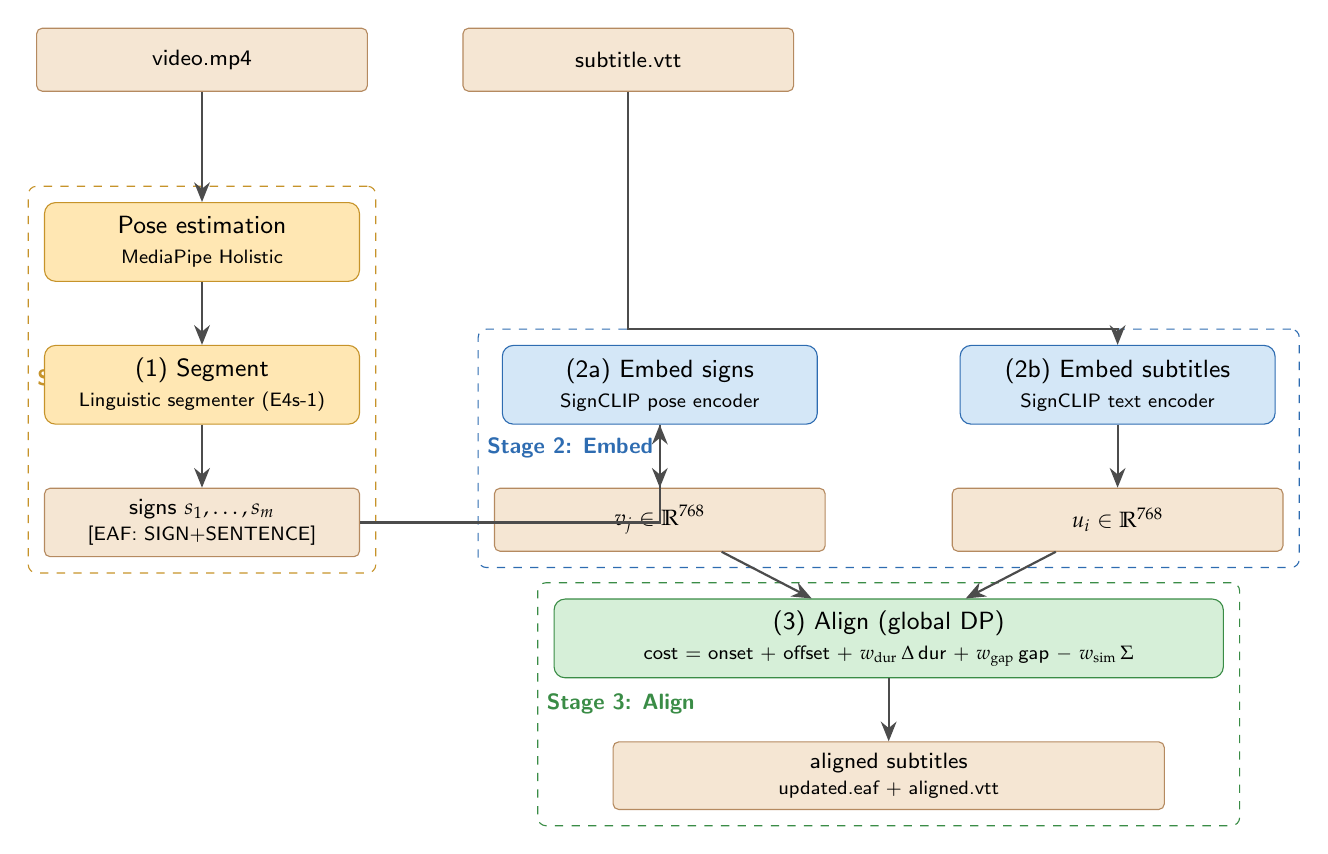
\begin{tikzpicture}[node distance=10mm and 12mm]
  % data inputs
  \node[data]                                    (vid)   {video.mp4};
  \node[data, right=of vid]                      (subs)  {subtitle.vtt};

  % segmentation
  \node[seg, below=14mm of vid, minimum width=40mm]   (pose) {Pose estimation\\\scriptsize MediaPipe Holistic};
  \node[seg, below=8mm of pose, minimum width=40mm]   (seg)  {(1) Segment\\\scriptsize Linguistic segmenter (E4s-1)};
  \node[data, below=8mm of seg, minimum width=40mm]   (signs){signs $s_1,\dots,s_m$\\\scriptsize {[}EAF: SIGN+SENTENCE{]}};

  % embedding (signs)
  \node[emb, right=18mm of seg, minimum width=40mm]   (embS) {(2a) Embed signs\\\scriptsize SignCLIP pose encoder};
  % embedding (text)
  \node[emb, right=18mm of embS, minimum width=40mm]  (embT) {(2b) Embed subtitles\\\scriptsize SignCLIP text encoder};

  % shared latent
  \node[data, below=8mm of embS, minimum width=42mm]  (vEmb) {$v_j \in \mathbb{R}^{768}$};
  \node[data, below=8mm of embT, minimum width=42mm]  (uEmb) {$u_i \in \mathbb{R}^{768}$};

  % alignment
  \node[ali, below=10mm of $(vEmb)!0.5!(uEmb)$, minimum width=85mm]
        (align){(3) Align (global DP)\\\scriptsize cost = onset + offset + $w_{\rm dur}$\,$\Delta$\,dur + $w_{\rm gap}$\,gap $-$ $w_{\rm sim}$\,$\Sigma$};

  % output
  \node[data, below=8mm of align, minimum width=70mm] (out){aligned subtitles\\\scriptsize updated.eaf + aligned.vtt};

  % arrows
  \draw[flow] (vid)   -- (pose);
  \draw[flow] (pose)  -- (seg);
  \draw[flow] (seg)   -- (signs);
  \draw[flow] (signs.east) -| (embS.south);
  \draw[flow] (subs.south) |- ([yshift=2mm]embT.north) -- (embT);
  \draw[flow] (embS) -- (vEmb);
  \draw[flow] (embT) -- (uEmb);
  \draw[flow] (vEmb) -- (align);
  \draw[flow] (uEmb) -- (align);
  \draw[flow] (align) -- (out);

  % background banner labels
  \begin{scope}[on background layer]
    \node[draw=stageSegBd, dashed, fit=(pose)(seg)(signs), inner sep=2mm,
          rounded corners=3pt, label={[legend, anchor=west, text=stageSegBd]
          west:\textbf{Stage 1: Segment}}] {};
    \node[draw=stageEmbBd, dashed, fit=(embS)(embT)(vEmb)(uEmb), inner sep=2mm,
          rounded corners=3pt, label={[legend, anchor=west, text=stageEmbBd]
          west:\textbf{Stage 2: Embed}}] {};
    \node[draw=stageAlignBd, dashed, fit=(align)(out), inner sep=2mm,
          rounded corners=3pt, label={[legend, anchor=west, text=stageAlignBd]
          west:\textbf{Stage 3: Align}}] {};
  \end{scope}
\end{tikzpicture}
\caption{The three-stage SEA architecture as described in the paper. Yellow
boxes are the segmentation pipeline (pretrained), blue boxes are the SignCLIP
encoders (pretrained, dual-tower), and the green box is the new contribution:
a global DP that picks a contiguous span of signs for every subtitle.}
\label{fig:sea-arch}
\end{figure}

\subsection{Why this works as a universal recipe}
The paper makes three architectural points worth quoting.
\begin{itemize}[leftmargin=1.5em]
  \item Sign \emph{segmentation} models trained on one sign language transfer
        zero-shot to others, because they classify motion primitives rather
        than meaning. Moryossef et al.\ 2023 report 0.76 ROC-AUC on French
        Sign Language despite training on DGS.
  \item SignCLIP, the embedding model, is pretrained \emph{multilingually} on
        SpreadtheSign (41 sign languages on the video side; English on the
        text side). Language-specific finetuning gives a further boost when
        in-domain data is available, but is not required.
  \item The DP \emph{global} optimum has access to every sign in the episode,
        not a 20-second window, so it makes consistent decisions when one
        subtitle's signs are immediately followed by another's, and it does
        not need a separate DTW post-processing pass.
\end{itemize}


\section{The Segmentation Model in Detail}
\label{sec:paper-seg}

The paper adopts the linguistic segmentation model of Moryossef et al.\ 2023
(\emph{``Linguistically Motivated Sign Language Segmentation''}). Trained on
$\sim$73\,h of annotated DGS data from the Public DGS Corpus, it ingests
MediaPipe Holistic poses and emits a per-frame BIO tag (\textsc{B}eginning,
\textsc{I}nside, \textsc{O}utside) via a small bidirectional LSTM. The
specific checkpoint used is \texttt{model\_E4s-1.pth} (\texttt{E4s-1}), with
two scalar decoding parameters that turn per-frame probabilities into discrete
spans:
\begin{description}[leftmargin=1.6em,style=nextline]
  \item[\texttt{b-threshold} (range 0--100)] Probability above which a frame
  is treated as the boundary between two adjacent signs. Lower values
  encourage finer segmentation. The paper finds optimal values of 30 (BOBSL)
  and 20--40 across other datasets.
  \item[\texttt{o-threshold} (range 0--100)] Probability above which a frame
  is treated as outside signing (a pause). The paper uses 30--50.
\end{description}

\paragraph{Why this segmenter rather than newer ones?} The paper compares
several alternatives in its ablation study (its Table 4): the BSL-Corpus
trained models of Renz et al.\ 2021a/b achieve higher \emph{segmentation} F1
on BSLCP (47.71 vs.\ 31.13) but \emph{lower downstream alignment} F1 on BOBSL
(57.98 vs.\ 66.24). The paper attributes this to (i) a domain gap between
BSLCP and BOBSL, (ii) Renz et al.'s tendency to produce signing-positives on
non-signing frames, and (iii) the fact that downstream alignment seems to
benefit from \emph{slightly over-segmented} sub-sign units. SEA therefore
sticks with Moryossef's DGS-trained model. Even fine-tuning on BSLCP with
negative-sampling (\emph{Segmentation-BSLCP}, the paper's best segmenter at
F1 52.09) actually \emph{decreases} alignment quality (63.61 instead of
66.24).

\paragraph{Implementation detail relevant to this workspace.} The CLI used is
\texttt{pose\_to\_segments}, distributed from
\texttt{github.com/J22Melody/segmentation@bsl}. It writes ELAN \texttt{.eaf}
files containing two tiers: \texttt{SIGN} (per-sign annotations) and
\texttt{SENTENCE} (groups of adjacent signs forming a phrase).


\section{The Embedding Model in Detail (SignCLIP)}
\label{sec:paper-emb}

SignCLIP (Jiang et al., EMNLP~2024) is a CLIP-style dual encoder. The text
branch is a BERT-like transformer; the sign branch is initialised from the
same BERT weights and adapted to take a sequence of MediaPipe pose frames
instead of sub-words. Both branches output 768-dim L2-normalised vectors and
are trained with a contrastive InfoNCE loss between aligned pairs.

\paragraph{Pretraining (\emph{SignCLIP-multilingual}).} The base checkpoint
used by SEA is \texttt{baseline\_temporal} (codename \texttt{E7.2}), pretrained
on SpreadtheSign---41 sign languages on the video side; English on the text
side---hence the language-tag prepending convention
\texttt{<en> <bfi>} (BSL/English), \texttt{<en> <ase>} (ASL/English),
\texttt{<de> <sgg>} (DSGS/German). The text encoder thus speaks a sort of
``language pair'' protocol: the first tag is the spoken-language ISO code,
the second is the sign-language ISO code.

\paragraph{Language-specific finetuning.} The paper produces three additional
checkpoints by finetuning \emph{SignCLIP-multilingual} on different language-
specific corpora:
\begin{itemize}[leftmargin=1.5em]
  \item \emph{SignCLIP-BSL}: $\sim$3.5\,M sign spottings from BOBSL
        (Momeni et al., 2022), using a contrastive text objective over
        8{,}697 distinct signs.
  \item \emph{SignCLIP-ASL}: $\sim$200\,K examples aggregated from PopSign
        (Starner et al., 2023), ASL Citizen (Desai et al., 2023), and
        Sem-Lex (Kezar et al., 2023). Glosses are normalised to lowercase
        without variations.
  \item \emph{SignCLIP-Suisse}: 16{,}213 lexical items from Signsuisse, each
        paired with an example sentence (M{\"u}ller et al., 2023).
\end{itemize}
Total finetuning time is reported as ``less than 3 days on an NVIDIA RTX
A6000 GPU with 48\,GB of memory''.

\paragraph{ISLR$\,\leftrightarrow\,$alignment correlation.} The paper observes
a consistent positive correlation between an embedding's
isolated-sign-language-recognition (ISLR) score and its downstream alignment
F1. For BSL: SignCLIP-multilingual gets 0.5 ISLR and 66.70 F1@0.50;
SignCLIP-BSL gets 43.0 ISLR and 72.78 F1@0.50. For ASL on PopSign: 3.0/35.51
vs.\ 84.3/38.32. The slope is much smaller for ASL because How2Sign signing
is unusually continuous (no prosodic pauses), reducing the value of any
boundary-related cue.


\section{The Alignment Algorithm in Detail (Paper Description)}
\label{sec:paper-align}

\subsection{Cost function}
For a candidate assignment of cue $t_i$ to a contiguous span of signs
$\{s_l, \ldots, s_r\}$, the paper defines a per-pair cost
\begin{align}
\phi(t_i,\,s_{l:r}) \;=\;
& \bigl|\mathrm{start}(t_i) - \mathrm{start}(s_l)\bigr|
  + \bigl|\mathrm{end}(t_i)   - \mathrm{end}(s_r)\bigr| \nonumber\\
& + w_{\mathrm{dur}} \,\bigl|\,\mathrm{dur}(t_i) - \mathrm{dur}(s_{l:r})\,\bigr|
  + w_{\mathrm{gap}} \,G(l,r) \nonumber\\
& - w_{\mathrm{sim}} \,\Sigma(i;\,l,r),
\label{eq:cost}
\end{align}
where the inter-sign-gap term is
\[
G(l,r) \;=\;
\sum_{j=l}^{r-1} \max\bigl(0,\;\mathrm{start}(s_{j+1}) - \mathrm{end}(s_j)\bigr),
\]
and the cumulative similarity term is
$\Sigma(i;\,l,r) = \sum_{j=l}^{r} M_{ij}$
with $M$ the (locality-masked, row-softmax-normalised) similarity matrix.
Setting $w_{\mathrm{sim}} = 0$ recovers the timing-only \emph{Segment and
Align} variant; with $w_{\mathrm{sim}} > 0$ one obtains \emph{Segment, Embed,
and Align}.

\subsection{Locality constraint and softmax normalisation}
For every cue row $i$, the paper keeps only the
\texttt{win\_size}${} = 50$ temporally-nearest signs (others masked to 0)
and then row-softmax-normalises with temperature $\tau = 10$. The result is
``a matrix of values concentrated around the temporal diagonal'' (paper, \S
A.2). Without this masking the DP would happily pull captions across the
entire episode.

\subsection{Global DP recurrence}
The DP table is
\[
\mathrm{dp}[i,j] \;=\;
\min_{i-1 \le k < j} \mathrm{dp}[i-1, k] + \phi(t_i,\,s_{k:j-1}),
\quad \mathrm{dp}[0,0]=0,\; \mathrm{dp}[0,j>0]=\infty.
\]
Crucially, the algorithm does \emph{not} require the last cue to land on the
last sign. After filling the table, the optimal end-point is
$j^\star = \arg\min_{0\le j \le m} \mathrm{dp}[n, j]$, and backtracking
recovers the assignment. This is essential because false-positive ``signing''
often appears at the very end of episodes (e.g.\ closing visuals).

\subsection{Sub-group refinement}
After the global DP picks span boundaries $[l_i, r_i]$ for each cue, a local
post-processing pass splits the span into maximal sub-spans whose internal
gaps are all $\le$ \texttt{max\_gap}, then chooses the sub-span with the
lowest local cost. This is what the paper's pseudocode calls
\texttt{pick\_best(subgroups, ...)} (line 30 of Appendix Figure 4).

\subsection{Pre- and post-DP fixed offsets}
Both before \emph{and} after the DP, every cue is shifted by a pair of fixed
offsets $(\delta_s, \delta_e)$ found by random search. The paper observes
that ``a fixed 1-second offset applied after the DP process is always useful
in the datasets evaluated''---a regularity attributed to annotators tending
to leave subtitles on slightly past the end of signing.

\subsection{Random parameter search}
For each dataset with a training set, the paper runs up to $10{,}000$ random
combinations on 128 CPU workers ($\sim$1 day of search) under the
\emph{Segment and Align} setting; the best combination is then inherited for
\emph{Segment, Embed, and Align}, with only $w_{\mathrm{sim}}$ re-tuned. The
authoritative parameter values from the paper's Appendix Table 5 are
reproduced in Table~\ref{tab:paper-params}.

\begin{table}[h]
\centering
\small
\begin{tabular}{lrrrr}
\toprule
\textbf{Parameter} & \textbf{BOBSL} & \textbf{How2Sign} & \textbf{WMT-SLT} & \textbf{SwissSLi} \\
\midrule
Start offset before DP                & 2.6  & 1.3  & 1.4  & 0.49 \\
End offset before DP                  & 2.1  & 1.5  & 1.6  & 0.56 \\
Start offset after DP                 & 0.0  & 0.0  & 0    & 0    \\
End offset after DP                   & 1.0  & 1.0  & 1    & 1    \\
\texttt{b-threshold} for segmentation & 30   & 40   & 20   & 20   \\
\texttt{o-threshold} for segmentation & 50   & 50   & 30   & 30   \\
\texttt{win\_size}                    & 50   & 50   & 50   & 50   \\
\texttt{max\_gap} (s)                 & 10   & 8    & 6    & 6    \\
$w_{\mathrm{dur}}$                    & 1    & 5    & 0.5  & 0.5  \\
$w_{\mathrm{gap}}$                    & 5    & 0.8  & 5    & 5    \\
$w_{\mathrm{sim}}$                    & 10   & 10   & 5    & 1    \\
\bottomrule
\end{tabular}
\caption{Best per-dataset parameter settings reported in the SEA paper
(Appendix Table 5). Offsets and gaps are in seconds.}
\label{tab:paper-params}
\end{table}


\section{Datasets and Baselines (from the Paper)}
\label{sec:paper-data}

\begin{table}[h]
\centering
\small
\begin{tabularx}{\linewidth}{lXrrrr}
\toprule
\textbf{Dataset} & \textbf{Languages / Source} & \textbf{Episodes} & \textbf{Subs} & \textbf{Hours} & \textbf{Offsets (s)} \\
\midrule
BOBSL          & BSL/English, mixed BBC programmes (interpreted)       & 55    & 31{,}479 & $\sim$46  & 2.70/2.70 \\
How2Sign       & ASL/English, studio-recorded re-signing               & 2{,}528 & 35{,}191 & $\sim$80 & 1.57/2.13 \\
WMT-SLT~SRF    & DSGS/German, live news interpretation                 & 29    & 7{,}071  & $\sim$16  & 1.06/1.75 \\
SwissSLi mit.\ & DSGS/German, deaf-translated programme (offline)      & 14    & 554      & $\sim$1   & 0.49/0.56 \\
\bottomrule
\end{tabularx}
\caption{The four sign-language datasets in the SEA evaluation
(Paper Table 1). Offsets are the median (or mean for BOBSL) shift between
audio-aligned and human-aligned subtitles, used by the
\emph{Original$^{+}$} baseline.}
\label{tab:paper-datasets}
\end{table}

\paragraph{Baselines.}
\begin{itemize}[leftmargin=1.5em]
  \item \emph{Original}: the audio-aligned subtitles shipped with the dataset.
  \item \emph{Original$^{+}$}: \emph{Original} plus a fixed offset (median
        shift on the training set).
  \item \emph{SAT} (Bull et al., 2021): an end-to-end transformer trained on
        17.7\,h of manually aligned BSL data. Uses BERT for text and I3D for
        video, cross-attended in an encoder-decoder, predicts frame-level
        labels in a 20-second window, and resolves overlap with DTW.
  \item \emph{SAT$^{+}$} (Jang et al., 2025): SAT plus three improvements:
        grammatical preprocessing of subtitles, a selective alignment loss
        with negative sampling, and iterative self-training with refined
        pseudo-labels. Current SOTA on BOBSL among end-to-end methods.
\end{itemize}

\paragraph{Evaluation metric: F1@0.50.} A predicted subtitle is counted as
correct when its predicted segment overlaps the ground truth with
intersection-over-union (IoU) $\ge 0.50$. The paper prefers F1 over
frame-accuracy because SEA does not predict at the frame level.

\paragraph{Headline result (paper Table 2).} SEA is SOTA on every test set.
Selected numbers reproduced below; bold = best in column.

\begin{table}[h]
\centering
\small
\renewcommand{\arraystretch}{1.1}
\resizebox{\linewidth}{!}{%
\begin{tabular}{lcccc}
\toprule
& \textbf{BOBSL Test} & \textbf{How2Sign Test} & \textbf{WMT-SLT Test} & \textbf{SwissSLi Test} \\
\midrule
Original                                             & 14.11 & 33.06 & 46.85 & 60.48 \\
Original$^{+}$                                       & 44.61 & 36.21 & 74.83 & ---   \\
SAT                                                  & 54.57 & ---   & 75.32 & ---   \\
SAT$^{+}$                                            & 63.81 & ---   & ---   & ---   \\
\midrule
\textbf{Segment and Align}                           & 49.58 & 36.17 & 76.83 & 84.19 \\
\textbf{Segment, Embed, and Align (multilingual)}    & 50.68 & 37.51 & 76.43 & \textbf{85.57} \\
\textbf{Segment, Embed, and Align (lang-finetuned)}  & 54.50 & \textbf{39.57} & \textbf{77.69} & 85.22 \\
\textbf{SignCLIP-BSL + SAT$^{+}$ subtitles}          & \textbf{65.68} & --- & --- & --- \\
\bottomrule
\end{tabular}}
\caption{F1@0.50 on the four test sets, paper Table~2 (test columns only).
SEA is SOTA on every test set; chaining SEA on top of SAT$^{+}$ gives a
further boost on BOBSL.}
\label{tab:paper-results}
\end{table}

\paragraph{Take-away from the paper.} (1) Even \emph{Segment and Align}
without any embedding already beats SAT on BOBSL (49.58 vs.\ 54.57---wait,
actually SAT is higher here; the paper notes SEA's gain is mostly on
\emph{Original$^{+}$} and on cross-language datasets). (2) Adding SignCLIP
similarity always helps; language-specific finetuning helps further when
in-domain data is available. (3) SEA can be \emph{chained} with SAT$^{+}$:
take SAT$^{+}$'s output as the prior subtitle locations and let SEA refine
them, gaining $\sim$2 points on BOBSL. (4) On How2Sign, alignment is
inherently hard because random non-subtitled signing appears at episode
ends; SEA still improves over the baseline, but the gain is smaller.

\paragraph{Pseudocode (paper Appendix Figure 4).} The full SEA algorithm
fits in $\sim$30 lines of Python:

\begin{lstlisting}
# Step 1 -- Segment
signs = segmenter(video)
# Step 2 -- Embed
v_emb = embed_sign(signs)
t_emb = embed_text(subtitles)
sim_matrix = dot_product(t_emb, v_emb)
# Step 3 -- Align
def cost(cue, span):
    a = abs(cue.start - span.start)
    b = abs(cue.end - span.end)
    c = abs(cue.duration - span.duration)
    d = compute_internal_gap(span)
    e = compute_total_similarity(cue, span)
    return a + b + w_dur*c + w_gap*d - w_sim*e

sim_matrix = zero_out(sim_matrix, win_size)
sim_matrix = softmax_normalize(sim_matrix)

dp     = aligner(signs, subtitles, cost, sim_matrix)
bounds = backtrack(dp)

# Refinement on internal gap
for i in range(len(subtitles)):
    group     = signs[bounds[i]:bounds[i+1]]
    subgroups = split_on_gap(group, max_gap)
    alignments[i] = pick_best(subgroups, subtitles[i], cost)

# Update timestamps
for i in range(len(subtitles)):
    subtitles[i].start = alignments[i][0].start
    subtitles[i].end   = alignments[i][-1].end
\end{lstlisting}

\clearpage
% ============================================================
\part{This Workspace --- TSL Pipeline}
% ============================================================

\section{Project Goals on Thai Sign Language}

This workspace adapts SEA to Thai Sign Language (TSL). The codebase is a fork
of \href{https://github.com/J22Melody/SEA}{J22Melody/SEA} (commit
\texttt{5aaf27d}) plus the SignCLIP encoder from
\href{https://github.com/J22Melody/fairseq}{J22Melody/fairseq}, with a small
set of patches required to make both run on Windows and to support multi-model
live embedding (\S\ref{sec:patches}).

\subsection{Two concrete tasks formulated for TSL}
\paragraph{Task~1 (focus of this report).} Take 172 CC cues with
audio-aligned timestamps and produce visually-aligned timestamps that match
the 119 expert annotations (\texttt{CC\_Aligned}) produced by a human
researcher.

\paragraph{Task~2 (future work).} Expand each sentence-level Gloss
annotation (119 entries) into the finer 852 per-sign \texttt{Gloss\_Labeling}
entries automatically. The workspace contains the necessary infrastructure
(token-level similarity is already implemented in
\texttt{align\_similarity.py} via \texttt{--tokenize\_text\_embedding}); only
the DP needs to be specialised to operate inside each sentence's bounds.

\subsection{The single TSL example used throughout}
The lecture video \emph{``The Comparison and Ordering''} (in Thai), 11~min
07~s, 1920$\times$1080@60\,fps. The four ground-truth tiers in its EAF are:

\begin{table}[h]
\centering
\small
\begin{tabularx}{\linewidth}{lXr}
\toprule
\textbf{Tier} & \textbf{Content} & \textbf{Count} \\
\midrule
\texttt{CC}             & Raw Thai captions, audio-synced (input)        & 172 \\
\texttt{CC\_Aligned}    & Manually re-aligned captions \emph{(GT)}       & 119 \\
\texttt{Gloss}          & Sign-language gloss strings, sentence-level    & 119 \\
\texttt{Gloss Labeling} & Per-sign gloss annotation                      & 852 \\
\bottomrule
\end{tabularx}
\end{table}


\section{Pipeline Walkthrough --- Step by Step}
\label{sec:walkthrough}

For each step we state \textbf{(a)} \emph{what the step is},
\textbf{(b)} \emph{how it is done in this workspace} (commands, parameters,
code references), \textbf{(c)} \emph{the algorithmic detail} worth knowing,
and \textbf{(d)} \emph{the artefact that the step produces}.

% ============================================================
% Workspace pipeline diagram with all artefacts
% ============================================================
\begin{figure}[ht]
\centering
\resizebox{\linewidth}{!}{%
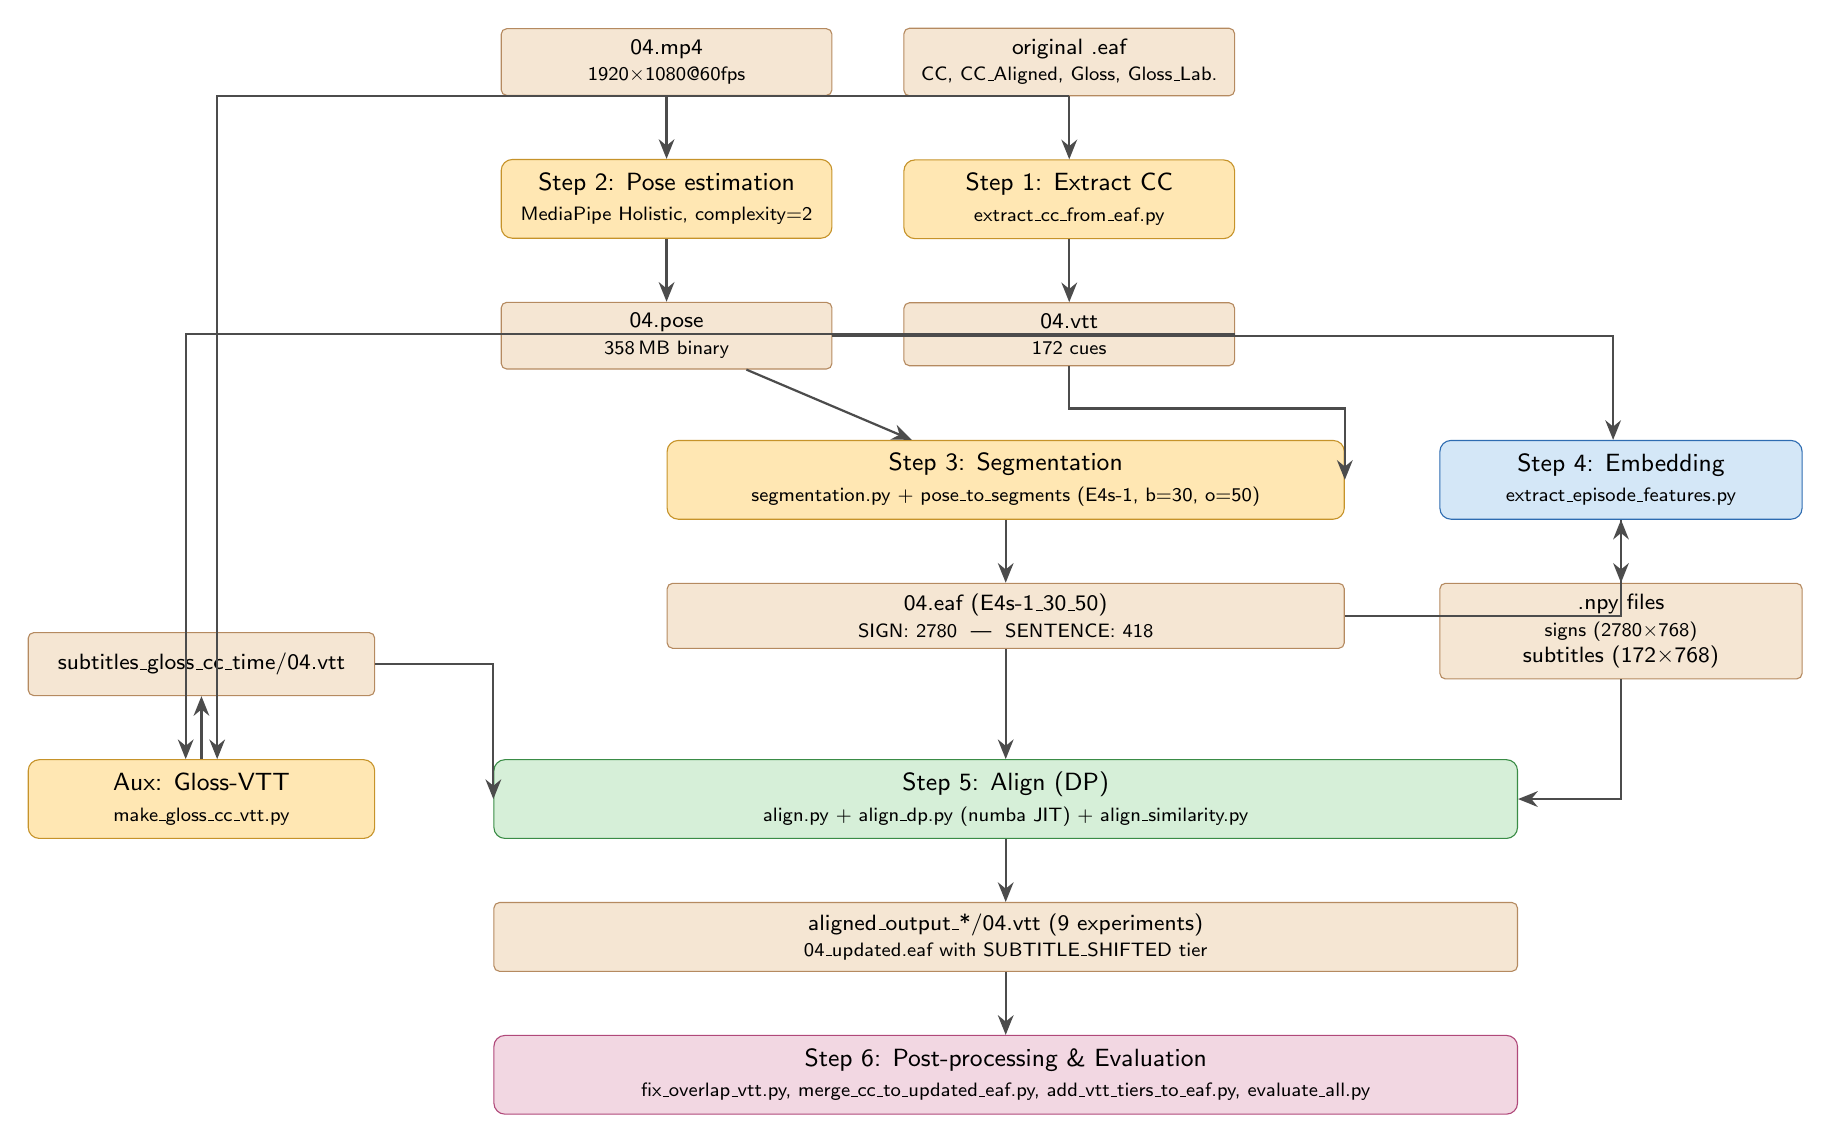
\begin{tikzpicture}[node distance=8mm and 9mm, scale=1, transform shape]
  % --- top row: inputs
  \node[data]                              (mp4)  {04.mp4\\\scriptsize 1920$\times$1080@60fps};
  \node[data, right=of mp4]                (eaf)  {original .eaf\\\scriptsize CC, CC\_Aligned, Gloss, Gloss\_Lab.};

  % step 1: extract CC
  \node[seg, below=of eaf, minimum width=42mm] (s1) {Step 1: Extract CC\\\scriptsize extract\_cc\_from\_eaf.py};
  \node[data, below=of s1] (vtt) {04.vtt\\\scriptsize 172 cues};

  % step 2: pose
  \node[seg, below=of mp4, minimum width=42mm] (s2) {Step 2: Pose estimation\\\scriptsize MediaPipe Holistic, complexity=2};
  \node[data, below=of s2] (pose) {04.pose\\\scriptsize 358\,MB binary};

  % step 3: segmentation (centred under poses)
  \node[seg, below=14mm of pose, minimum width=86mm, anchor=west, xshift=0mm]
        (s3) {Step 3: Segmentation\\\scriptsize segmentation.py + pose\_to\_segments (E4s-1, b=30, o=50)};
  \node[data, below=of s3, minimum width=86mm] (segeaf) {04.eaf (E4s-1\_30\_50)\\\scriptsize SIGN: 2780~~|~~SENTENCE: 418};

  % step 4: embedding (right column)
  \node[emb, right=12mm of s3, minimum width=46mm] (s4) {Step 4: Embedding\\\scriptsize extract\_episode\_features.py};
  \node[data, below=of s4, minimum width=46mm] (npys) {.npy files\\\scriptsize signs (2780$\times$768)\\subtitles (172$\times$768)};

  % step 5: align
  \node[ali, below=14mm of segeaf, minimum width=130mm]
        (s5){Step 5: Align (DP)\\\scriptsize align.py + align\_dp.py (numba JIT) + align\_similarity.py};
  \node[data, below=of s5, minimum width=130mm] (aligned)
        {aligned\_output\_*/04.vtt (9 experiments)\\\scriptsize 04\_updated.eaf with SUBTITLE\_SHIFTED tier};

  % step 6: postprocess
  \node[post, below=of aligned, minimum width=130mm]
        (s6){Step 6: Post-processing \& Evaluation\\\scriptsize fix\_overlap\_vtt.py, merge\_cc\_to\_updated\_eaf.py, add\_vtt\_tiers\_to\_eaf.py, evaluate\_all.py};

  % aux gloss VTT
  \node[seg, left=15mm of s5, minimum width=44mm, yshift=0mm]
        (gloss){Aux: Gloss-VTT\\\scriptsize make\_gloss\_cc\_vtt.py};
  \node[data, above=of gloss, minimum width=44mm] (gvtt){subtitles\_gloss\_cc\_time/04.vtt};

  % --- arrows
  \draw[flow] (mp4)  -- (s2);
  \draw[flow] (s2)   -- (pose);
  \draw[flow] (eaf)  -- (s1);
  \draw[flow] (s1)   -- (vtt);
  \draw[flow] (pose) -- (s3);
  \draw[flow] (vtt.south) |- ([yshift=4mm]s3.north -| s3.east) -- (s3.east);
  \draw[flow] (s3)   -- (segeaf);
  \draw[flow] (segeaf.east) -| (s4);
  \draw[flow] (pose.east)   -| ([xshift=-1mm]s4.north);
  \draw[flow] (s4)          -- (npys);
  \draw[flow] (segeaf)      -- (s5);
  \draw[flow] (npys.south)  |- (s5.east);
  \draw[flow] (vtt.east) -| ([xshift=-2mm]gloss.north);
  \draw[flow] (eaf.south) -| ([xshift=2mm]gloss.north);
  \draw[flow] (gloss) -- (gvtt);
  \draw[flow] (gvtt.east) -| ([yshift=4mm]s5.west) -- (s5.west);
  \draw[flow] (s5)        -- (aligned);
  \draw[flow] (aligned)   -- (s6);
\end{tikzpicture}%
}
\caption{End-to-end workspace pipeline. Yellow = ingestion / segmentation;
blue = SignCLIP embedding; green = global DP alignment; pink = post-processing
and evaluation; parchment = data artefacts (with their actual sizes/counts in
the workspace). Boxes labelled ``\emph{Aux}'' are tools developed in this
workspace, not part of upstream SEA.}
\label{fig:full-pipeline}
\end{figure}

% --------------------------------------------------------------
\subsection{Step 0: Environment}
\label{sec:step0}

\paragraph{What.} A Python 3.11 virtual environment with PyTorch (CUDA 12.8
for the local NVIDIA RTX 5060\,Ti, Blackwell, sm\_120), MediaPipe pinned at
\texttt{0.10.21}, the BSL-branch sign segmenter, plus standard subtitle/EAF
libraries.

\paragraph{Hardware.} Intel Core Ultra 7 265K (20 cores), 64\,GB RAM, RTX
5060\,Ti with 17.1\,GB VRAM, Windows 11.

\paragraph{Install (one-time).}
\begin{lstlisting}
python -m venv venv
venv\Scripts\activate
pip install pysrt webvtt-py lxml numpy pympi-ling
pip install "mediapipe==0.10.21" pose-format
pip install beartype numba tqdm scikit-learn tabulate
pip install "git+https://github.com/J22Melody/segmentation@bsl"
pip install --force-reinstall torch \
    --index-url https://download.pytorch.org/whl/cu128
\end{lstlisting}

\paragraph{Pitfalls actually hit during setup.}
\begin{itemize}[leftmargin=1.5em]
  \item \textbf{MediaPipe must be 0.10.21}: 0.10.22+ broke
  \texttt{videos\_to\_poses}.
  \item \textbf{PyTorch \texttt{cu128}} is mandatory for sm\_120; cu126
  silently falls back to CPU on Blackwell.
  \item \texttt{numba} is required by the JIT-compiled DP inner loop. The
  fork has a fallback path that runs plain Python if numba is missing
  (\texttt{align\_dp.py} lines 4--7).
  \item \texttt{video\_ids.txt} must be UTF-8 without BOM. \texttt{echo 04 >
  video\_ids.txt} on Windows produces UTF-16 BOM and crashes the segmenter.
\end{itemize}

\paragraph{Result.} A reproducible environment at \texttt{SEA/venv/}.


% --------------------------------------------------------------
\subsection{Step 1: Extract CC from EAF $\rightarrow$ WebVTT}
\label{sec:step1}

\paragraph{What.} The original Thai annotation file is in ELAN's XML-based
EAF format. SEA expects subtitles in WebVTT (or SRT). This step parses the
\texttt{CC} tier from the EAF and writes a standard \texttt{.vtt}.

\paragraph{Code.} \texttt{example\_alignment/extract\_cc\_from\_eaf.py}.

\paragraph{Algorithm.}
\begin{enumerate}[leftmargin=1.5em]
  \item Parse the EAF with \texttt{xml.etree.ElementTree}.
  \item Build a dictionary \texttt{TIME\_SLOT\_ID $\to$ seconds} (the EAF
        stores times in milliseconds).
  \item Locate the \texttt{TIER} whose \texttt{TIER\_ID="CC"}, then for every
        \texttt{ANNOTATION} read \texttt{TIME\_SLOT\_REF1/REF2} and the
        \texttt{ANNOTATION\_VALUE} text.
  \item Sort the resulting cues by start time and emit standard WebVTT.
\end{enumerate}

\paragraph{Conversion formula.}
$t_\text{vtt} = \mathrm{TIME\_VALUE}\,\mathrm{[ms]}/1000$, formatted to
\texttt{HH:MM:SS.mmm}. End times shorter than start times (occasional EAF
artefact) are swapped.

\paragraph{Run.}
\begin{lstlisting}
python extract_cc_from_eaf.py "...11.07 .eaf" 04.vtt
\end{lstlisting}

\paragraph{Result (verified).} \texttt{04.vtt} containing exactly \textbf{172}
cues. The first two cues (rendered in English) read:
\begin{lstlisting}
WEBVTT

1
00:00:00.040 --> 00:00:31.890
[opening music]

2
00:00:34.030 --> 00:00:36.210
(Teacher) Hello everyone
\end{lstlisting}


% --------------------------------------------------------------
\subsection{Step 2: Pose Estimation}
\label{sec:step2}

\paragraph{What.} Convert the pixel-domain video into a sequence of human
skeletons. MediaPipe Holistic predicts 543 landmarks per frame: 33 body,
21$\times$2 hand, and 468 facial points. Working on poses (rather than
pixels) makes downstream sign processing language-agnostic.

\paragraph{Run.}
\begin{lstlisting}
videos_to_poses --format mediapipe --directory . \
  --additional-config="model_complexity=2,smooth_landmarks=false,refine_face_landmarks=true"
\end{lstlisting}

\paragraph{Why these settings.}
\begin{itemize}[leftmargin=1.5em]
  \item \texttt{model\_complexity=2}: highest accuracy. About 15 minutes of
        CPU time per 11-minute 60\,fps video.
  \item \texttt{smooth\_landmarks=false}: the segmenter is itself an LSTM that
        smooths frame-to-frame; pre-smoothing washes out boundaries.
  \item \texttt{refine\_face\_landmarks=true}: TSL uses face/lip non-manuals
        on roughly the same level as hand-shapes.
\end{itemize}

\paragraph{Result (verified).} \texttt{04.pose} (\textbf{358\,MB} binary).
Each frame stores 543 $(x,y,z,\text{conf})$ landmarks at 60\,fps for 668\,s,
i.e.\ approximately $668 \times 60 \times 543 \times 4 \approx 90$\,M float32
values plus metadata.


% --------------------------------------------------------------
\subsection{Step 3: Sign Segmentation}
\label{sec:step3}

\paragraph{What.} Cut the continuous pose stream into individual sign units
and group them into sentences. The output is an EAF with two tiers:
\texttt{SIGN} (one entry per individual sign) and \texttt{SENTENCE} (groups
of contiguous signs forming a phrase).

\paragraph{Model.} \texttt{model\_E4s-1.pth} (Section~\ref{sec:paper-seg}),
DGS-trained but transfers zero-shot.

\paragraph{Run.}
\begin{lstlisting}
cd SEA
python segmentation.py \
  --sign-b-threshold 30 --sign-o-threshold 50 --num_workers 1 \
  --video_ids ..\example_alignment\video_ids.txt \
  --pose_dir  ..\example_alignment \
  --save_dir  ..\example_alignment\segmentation_output \
  --video_dir ..\example_alignment
\end{lstlisting}
The output directory name encodes the model and thresholds:
\texttt{E4s-1\_30\_50}, so multiple parameter sweeps coexist.

\paragraph{Algorithmic flow inside \texttt{segmentation.py}.}
\begin{enumerate}[leftmargin=1.5em]
  \item Build the cartesian product of (\texttt{model}, \texttt{b-threshold},
        \texttt{o-threshold}) and the list of video IDs.
  \item For each combination, build a \texttt{pose\_to\_segments} command
        line with the proper \texttt{--pose}, \texttt{--elan}, \texttt{--video}
        and optional \texttt{--subtitles} arguments.
  \item Use \texttt{shlex.split} (rather than \texttt{shell=True}) to be
        Windows-safe, then run each task either sequentially or via
        \texttt{multiprocessing.Pool}.
\end{enumerate}

\paragraph{Workspace patches.}
\begin{itemize}[leftmargin=1.5em]
  \item Line 71 of \texttt{segmentation.py} was changed:
\begin{lstlisting}
# before (broken on Windows):
result = subprocess.run(cmd, shell=True)
# after (works on Windows):
result = subprocess.run(shlex.split(cmd), shell=False)
\end{lstlisting}
        \texttt{shlex.quote()} wraps every path in single quotes which
        \texttt{cmd.exe} does not strip; switching to \texttt{shlex.split}
        avoids the quoting layer entirely.
  \item Video paths are wrapped with \texttt{os.path.abspath()}.
\end{itemize}

\paragraph{Result (verified).}
\texttt{segmentation\_output/E4s-1\_30\_50/04.eaf} containing
\textbf{2{,}780} \texttt{SIGN} entries and \textbf{418} \texttt{SENTENCE}
entries. The XML contains 6{,}396 \texttt{TIME\_SLOT}s and 3{,}198
\texttt{ALIGNABLE\_ANNOTATION}s.


% --------------------------------------------------------------
\subsection{Step 4: Embedding (SignCLIP)}
\label{sec:step4}

\paragraph{What.} Embed each \texttt{SIGN} segment into a 768-dim vector and
embed each subtitle cue into the \emph{same} 768-dim space, so the two are
directly comparable by dot product.

\paragraph{Three checkpoint variants used here.}
\begin{itemize}[leftmargin=1.5em]
  \item \texttt{bsl} ($\to$ \texttt{bobsl\_finetune}): SignCLIP-multilingual
        finetuned on $\sim$3.5\,M BOBSL sign spottings.
  \item \texttt{multilingual} ($\to$ \texttt{baseline\_temporal}): the
        SpreadtheSign-pretrained base.
  \item \texttt{asl} ($\to$ \texttt{asl\_finetune}): finetuned on
        PopSign+ASL Citizen+Sem-Lex.
\end{itemize}

\paragraph{Run (BSL, signs).}
\begin{lstlisting}
python scripts_bsl/extract_episode_features.py \
  --video_ids ..\..\..\example_alignment\video_ids.txt \
  --mode=segmentation --model_name bsl --language_tag "<en> <bfi>" \
  --batch_size=32 \
  --pose_dir ..\..\..\example_alignment \
  --segmentation_dir ..\..\..\example_alignment\segmentation_output\E4s-1_30_50 \
  --save_dir ..\..\..\example_alignment\segmentation_embedding\sign_clip
\end{lstlisting}

\paragraph{Two modes.}
\begin{itemize}[leftmargin=1.5em]
  \item \texttt{--mode=segmentation}: reads the EAF from Step 3 plus the
        \texttt{.pose} file, extracts the pose frames inside each
        \texttt{SIGN} interval, runs them through the pose encoder, and
        writes an \texttt{(N\_signs, 768)} numpy array.
  \item \texttt{--mode=subtitle}: reads each cue's text, prepends the
        language tag, runs it through the text encoder, and writes
        \texttt{(M\_cues, 768)}.
\end{itemize}

\paragraph{Live (on-the-fly) embedding.} The custom flag
\texttt{--live\_embedding} in \texttt{align.py} (added by this fork) skips
the .npy step and embeds directly during alignment. With
\texttt{--tokenize\_text\_embedding}, each cue's text is split into words,
each word is encoded separately, and the token embeddings are pooled
(default: \texttt{max}) to form the cue embedding. This is the
\emph{word-level} variant used in experiments \texttt{C\_MULTI\_word} and
\texttt{D\_ASL\_word}.

\paragraph{Result (verified).}

\begin{table}[h]
\centering
\small
\begin{tabularx}{\linewidth}{lXr}
\toprule
\textbf{File} & \textbf{Variant} & \textbf{Verified shape} \\
\midrule
\texttt{segmentation\_embedding/sign\_clip/04.npy}            & BSL signs           & 2780$\times$768 \\
\texttt{segmentation\_embedding/sign\_clip\_multi/04.npy}     & Multilingual signs  & 2780$\times$768 \\
\texttt{segmentation\_embedding/sign\_clip\_asl/04.npy}       & ASL signs           & 2780$\times$768 \\
\texttt{subtitle\_embedding/sign\_clip/04.npy}                & BSL, CC text        & 172$\times$768  \\
\texttt{subtitle\_embedding/sign\_clip\_multi/04.npy}         & Multi, CC text      & 172$\times$768  \\
\texttt{subtitle\_embedding/sign\_clip\_multi\_gloss/04.npy}  & Multi, Gloss text   & 172$\times$768  \\
\texttt{subtitle\_embedding/sign\_clip\_asl/04.npy}           & ASL, CC text        & 172$\times$768  \\
\texttt{subtitle\_embedding/sign\_clip\_asl\_gloss/04.npy}    & ASL, Gloss text     & 172$\times$768  \\
\bottomrule
\end{tabularx}
\caption{All embedding artefacts present in this workspace.
Shapes confirmed by loading every \texttt{.npy} with \texttt{numpy};
\texttt{dtype} is \texttt{float32} for all of them.}
\label{tab:embeddings}
\end{table}


% --------------------------------------------------------------
\subsection{Auxiliary: Building the Gloss-text VTT}
\label{sec:gloss-vtt}

\paragraph{Why.} SignCLIP's text encoder was never trained on full Thai
sentences, but it does recognise sign-language gloss tokens (which look
much more like the gloss-style data the encoder saw at pretraining time).
Replacing the Thai sentence with the corresponding sign-language gloss makes
the similarity matrix more discriminative.

\paragraph{Code.} \texttt{example\_alignment/make\_gloss\_cc\_vtt.py}.

\paragraph{Algorithm.} For each CC cue $c$:
\begin{enumerate}[leftmargin=1.5em]
  \item Compute the temporal IoU with every \texttt{Gloss} entry $g$.
  \item Pick the one with the largest overlap.
  \item If overlap${}>0$: use $g.\text{text}$ (170 of 172 cues).
        Otherwise: fall back to the original CC text (2 cues).
\end{enumerate}
The CC start/end times are preserved so SEA still has to align from the
audio prior. The output is \texttt{subtitles\_gloss\_cc\_time/04.vtt}.

\paragraph{Result.} The CC text \emph{``We will study about comparison and
ordering of numbers''} becomes the gloss \emph{``HELLO STUDENT NEXT WHERE
LEARN COMPARISON ORDERING''}---short, sign-vocabulary-style, exactly the kind
of input SignCLIP's text encoder is happy with.


% --------------------------------------------------------------
\subsection{Step 5: Alignment via Dynamic Programming}
\label{sec:dp}

This is the technical heart of SEA. Driver:
\texttt{SEA/align.py}; DP recurrence: \texttt{SEA/align\_dp.py}; similarity
matrix: \texttt{SEA/align\_similarity.py}.

\subsubsection{Stage 5.1 --- Pre-shift bias}
SEA always begins by shifting every cue $c_i$ forward in time by a fixed
$(\delta_s, \delta_e)$. For BOBSL the paper finds $(2.6, 2.1)$\,s. For the
TSL example this workspace uses:
\begin{itemize}[leftmargin=1.5em]
  \item $(2.6, 2.1)$\,s for the standard CC-text profile (B1).
  \item $(1.8, 1.5)$\,s for the tuned CC-text profile (B2/B\_MULTI/D\_ASL).
  \item $(1.3, 1.0)$\,s for the Gloss-text profile (C\_MULTI/*\_gloss/*\_word).
\end{itemize}
The Gloss bias is smaller because the Gloss tier already has its timestamps
nudged closer to the visible signing.

\subsubsection{Stage 5.2 --- Candidate window}
For every cue $c_i$ the algorithm restricts attention to the
\texttt{dp\_window\_size} sign segments whose midpoints are temporally
closest to the cue midpoint (default 50; tuned profile uses 40). Anything
outside the window receives infinite cost and similarity 0. This locality
constraint bounds DP run-time to roughly $O(M \cdot W^2)$ instead of
$O(M \cdot N^2)$.

\subsubsection{Stage 5.3 --- Similarity matrix}
\label{sec:simmatrix}
With \texttt{--similarity\_measure sign\_clip\_embedding}, raw similarity
between cue $i$ and sign $j$ is the dot product of the two L2-normalised
embeddings:
\[
M^{0}_{ij} = \langle u_i, v_j\rangle, \quad u_i \in \mathbb{R}^{768},\;
v_j \in \mathbb{R}^{768}.
\]
The raw matrix is then locality-masked (entries outside the window-of-50
nearest signs zeroed) and row-softmax-normalised with temperature $\tau=10$:
\[
M_{ij} \;=\; \mathrm{softmax}_{\tau}\bigl(M^{0}_{i,\cdot}\bigr)_{j}\cdot 50.
\]
The factor $50$ scales the softmax outputs from probabilities back to
``count-like'' magnitudes so the similarity term is comparable in scale to
the timing terms in the cost function. Cumulative sums are pre-computed:
\[
S_{ij} = \sum_{j'=0}^{j-1} M_{ij'}, \quad
\Sigma(i;\,l,r) = S_{i,r+1} - S_{i,l},
\]
so the total similarity of any contiguous span $[l, r]$ can be retrieved in
$O(1)$.

\paragraph{Token-level variant (\texttt{--tokenize\_text\_embedding}).} Each
cue is encoded as several token vectors $u_i^{(1)}, \ldots, u_i^{(K)}$ and
similarity per sign is the max over tokens
$M^0_{ij} = \max_k \langle u_i^{(k)}, v_j\rangle$; the rest is identical.

\paragraph{Other measures.} \texttt{align\_similarity.py} also implements:
\begin{itemize}[leftmargin=1.5em]
  \item \texttt{cslr\_subtitle} / \texttt{cslr\_text}: hard-coded similarity
        matching pseudo-glosses (Raude et al., 2024) against the cue text.
  \item \texttt{text\_embedding}: replaces SignCLIP with a generic
        \texttt{all-MiniLM-L6-v2} sentence transformer; useful when no
        pose data is available but only segmenter outputs and gloss text.
  \item Three normalisation options: \texttt{softmax} (default),
        \texttt{z-score} sigmoid, or \texttt{sinkhorn} optimal-transport.
\end{itemize}

\subsubsection{Stage 5.4 --- Cost function}
\label{sec:cost}
Identical to Eq.~\eqref{eq:cost}. With the tuned-Gloss profile used by
\texttt{C\_MULTI}, the weights are $w_{\mathrm{dur}}{=}2$,
$w_{\mathrm{gap}}{=}8$, $w_{\mathrm{sim}}{=}6$,
\texttt{max\_gap}${=}6$\,s, \texttt{window\_size}${=}40$. These were
hand-tuned because the workspace did not run the paper's 10{,}000-iteration
random search; instead, parameters were adjusted iteratively by inspecting
the median offset and overlap rate after each run.

% ----------- Cost-function diagram -----------
\begin{figure}[h]
\centering
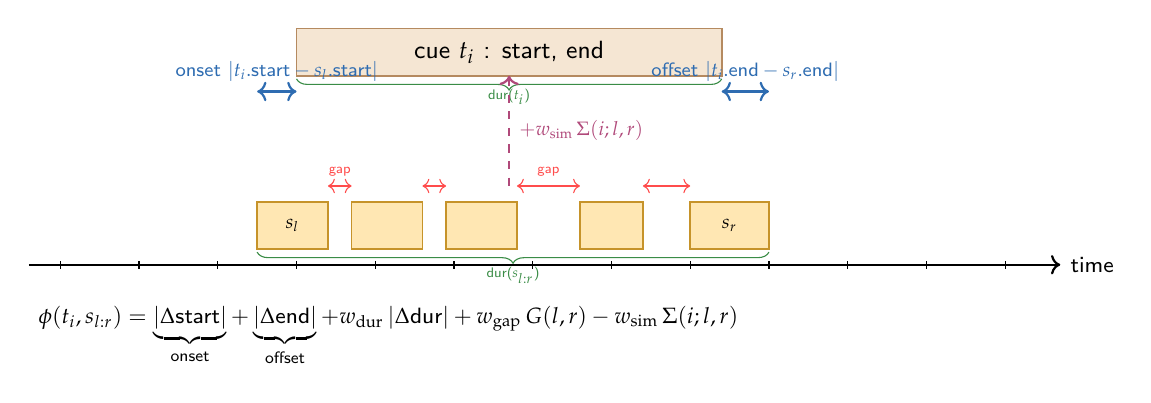
\begin{tikzpicture}[x=1cm,y=1cm,font=\sffamily]
  % time axis
  \draw[->,thick] (-0.4,0) -- (12.7,0) node[right]{\footnotesize time};
  \foreach \x in {0,1,...,12} \draw (\x,-0.05) -- (\x,0.05);

  % cue (subtitle) bar -- top
  \draw[fill=stageInput, draw=stageInputBd, line width=0.6pt]
    (3.0,2.4) rectangle (8.4,3.0);
  \node[font=\small\sffamily] at (5.7,2.7) {cue $t_i$ : start, end};

  % sign segments -- bottom
  \foreach \a/\b/\nm in {2.5/3.4/$s_l$, 3.7/4.6/{}, 4.9/5.8/{}, 6.6/7.4/{}, 8.0/9.0/$s_r$}
  {
     \draw[fill=stageSeg, draw=stageSegBd, line width=0.6pt] (\a,0.2) rectangle (\b,0.8);
     \node[font=\scriptsize\sffamily] at ({(\a+\b)/2},0.5) {\nm};
  }
  % gap arrows between adjacent signs
  \draw[<->, draw=red!70] (3.4,1.0) -- (3.7,1.0) node[midway,above,font=\tiny\sffamily,red!70] {gap};
  \draw[<->, draw=red!70] (4.6,1.0) -- (4.9,1.0);
  \draw[<->, draw=red!70] (5.8,1.0) -- (6.6,1.0) node[midway,above,font=\tiny\sffamily,red!70] {gap};
  \draw[<->, draw=red!70] (7.4,1.0) -- (8.0,1.0);

  % onset distance
  \draw[<->, draw=stageEmbBd, thick] (3.0,2.2) -- (2.5,2.2)
        node[midway,above,font=\scriptsize\sffamily,stageEmbBd]{onset $|t_i.\text{start}-s_l.\text{start}|$};
  % offset distance
  \draw[<->, draw=stageEmbBd, thick] (8.4,2.2) -- (9.0,2.2)
        node[midway,above,font=\scriptsize\sffamily,stageEmbBd]{offset $|t_i.\text{end}-s_r.\text{end}|$};

  % duration brackets
  \draw[decorate,decoration={brace,amplitude=4pt,mirror},stageAlignBd]
    (3.0,2.36) -- (8.4,2.36) node[midway,below,font=\tiny\sffamily,stageAlignBd]{dur($t_i$)};
  \draw[decorate,decoration={brace,amplitude=4pt,mirror},stageAlignBd]
    (2.5,0.16) -- (9.0,0.16) node[midway,below=2pt,font=\tiny\sffamily,stageAlignBd]{dur($s_{l:r}$)};

  % similarity reward (down-pointing dashed, between cue and span)
  \draw[<-, dashed, draw=stagePostBd, thick] (5.7,2.4) -- (5.7,1.0)
        node[midway,right,font=\scriptsize\sffamily,stagePostBd]{$+w_{\mathrm{sim}}\,\Sigma(i;l,r)$};

  % cost legend
  \node[anchor=west, font=\footnotesize\sffamily] at (-0.4,-0.9)
   {$\phi(t_i,s_{l:r}) = \underbrace{|\Delta\text{start}|}_{\text{onset}} +
      \underbrace{|\Delta\text{end}|}_{\text{offset}} +
      w_{\rm dur}\,|\Delta\text{dur}|+w_{\rm gap}\,G(l,r)-w_{\rm sim}\,\Sigma(i;l,r)$};
\end{tikzpicture}
\caption{Visual breakdown of the SEA cost function. The cue $t_i$ is matched
to the contiguous span of signs $s_l,\dots,s_r$. The cost penalises onset/offset
distance and duration mismatch (blue/green), inter-sign gaps inside the span
(red), and rewards (negative cost) the cumulative SignCLIP similarity along
the chosen row of the matrix (pink).}
\label{fig:cost-function}
\end{figure}

% ----------- DP recurrence diagram -----------
\begin{figure}[h]
\centering
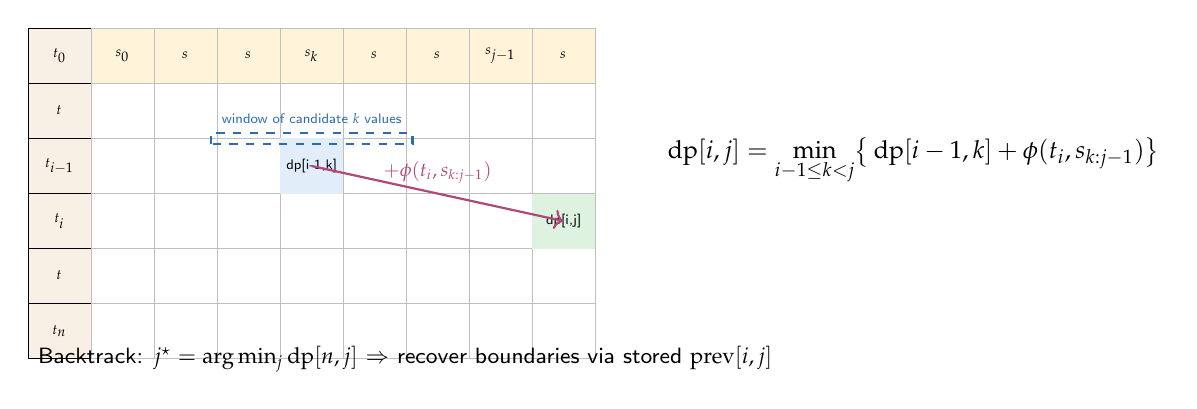
\begin{tikzpicture}[x=0.8cm,y=0.7cm,font=\sffamily]
  % column header (signs)
  \foreach \j/\lab in {0/0,1/{},2/{},3/k,4/{},5/{},6/{j-1},7/{}}
  {
    \fill[stageSeg!50] (\j,4) rectangle (\j+1,5);
    \draw (\j,4) rectangle (\j+1,5);
    \node[font=\tiny\sffamily] at (\j+0.5,4.5) {$s_{\lab}$};
  }
  % row header (cues)
  \foreach \i/\lab in {0/0,1/{},2/{i-1},3/i,4/{},5/n}
  {
    \fill[stageInput!60] (-1,4-\i) rectangle (0,5-\i);
    \draw (-1,4-\i) rectangle (0,5-\i);
    \node[font=\tiny\sffamily] at (-0.5,4.5-\i) {$t_{\lab}$};
  }
  % grid
  \foreach \i in {0,1,...,5}
    \foreach \j in {0,1,...,7}
    {
      \draw[gray!50] (\j,4-\i) rectangle (\j+1,5-\i);
    }
  % highlight dp[i-1,k]
  \fill[stageEmb!70] (3,2) rectangle (4,3);
  \node[font=\tiny\sffamily] at (3.5,2.5) {dp[i-1,k]};
  % highlight dp[i,j]
  \fill[stageAlign!80] (7,1) rectangle (8,2);
  \node[font=\tiny\sffamily] at (7.5,1.5) {dp[i,j]};
  % arrow from (i-1,k) to (i,j)
  \draw[->,thick,stagePostBd] (3.5,2.5) -- (7.5,1.5)
       node[midway, above, font=\scriptsize\sffamily, stagePostBd]
       {$+\phi(t_i,s_{k:j-1})$};

  % side label: minimum
  \node[anchor=west, font=\small\sffamily] at (9, 2.6)
    {$\mathrm{dp}[i,j]=\displaystyle\min_{i-1\le k<j}\bigl\{\,\mathrm{dp}[i-1,k]+\phi(t_i,s_{k:j-1})\bigr\}$};

  % candidate window indication
  \draw[stageEmbBd, thick, dashed]  (1.9,2.9) rectangle (5.1,3.1);
  \node[font=\tiny\sffamily,stageEmbBd, anchor=south] at (3.5,3.1) {window of candidate $k$ values};

  % bottom: backtrack
  \node[anchor=west, font=\footnotesize\sffamily] at (-1,-1.0)
    {Backtrack: $j^\star=\arg\min_j \mathrm{dp}[n,j]$ $\Rightarrow$ recover boundaries via stored $\mathrm{prev}[i,j]$};
\end{tikzpicture}
\caption{Dynamic programming recurrence. Each cell $\mathrm{dp}[i,j]$ stores
the minimum total cost of aligning the first $i$ cues to the first $j$
sign-segments. The transition from $\mathrm{dp}[i-1,k]$ to $\mathrm{dp}[i,j]$
adds the local cost $\phi$ of mapping cue $t_i$ to span $s_{k:j-1}$. The
candidate window restricts the search range of $k$ for locality. Final
backtracking starts at the column with minimum cost on the last row, not
necessarily the last column.}
\label{fig:dp-recurrence}
\end{figure}

\subsubsection{Stage 5.5 --- DP recurrence}
Identical to Section~\ref{sec:paper-align}. With $M=172$ and $N=2780$,
the table is $173 \times 2781$ entries, filled in a triple loop over
$i \in [1,M]$, $j \in [\,j_\text{lower},\,j_\text{upper}]$,
$k \in [i-1, j)$, where $[j_\text{lower}, j_\text{upper}]$ is the window
restriction. Backtracking starts at
$j^\star = \arg\min_j \mathrm{dp}[M, j]$ and walks backwards through
\texttt{prev}, recording one boundary index per cue.

\subsubsection{Stage 5.6 --- JIT inner loop}
\texttt{align\_dp.dp\_inner\_loop} is decorated with \texttt{numba.@njit}.
With JIT enabled, an 11-minute episode finishes in well under a second; the
plain-Python fallback (when LLVM is missing) takes roughly half a minute.

\subsubsection{Stage 5.7 --- Sub-group refinement}
After the global DP picks span boundaries $[l_i, r_i]$ for each cue, a local
post-processing pass splits the span into maximal sub-spans whose internal
gaps are all $\le$ \texttt{max\_gap}, then chooses the sub-span with the
lowest local cost. This prevents SEA from absorbing a long pause inside one
cue when in fact the next cue should start at the resumption.

\subsubsection{Stage 5.8 --- Post-shift and final write}
A second \texttt{shift\_cues} call applies the post-DP biases
$(\delta'_s, \delta'_e)$, defaulting to $(0, +1)$\,s. The result is written
as \texttt{aligned\_output\_*/04.vtt} via \texttt{utils.reconstruct\_vtt},
and as a \texttt{SUBTITLE\_SHIFTED} tier inside \texttt{04\_updated.eaf} via
\texttt{utils.write\_updated\_eaf}.

\subsubsection{Concrete invocation used in this workspace (B2)}
\begin{lstlisting}
python align.py --overwrite --mode=inference \
  --video_ids ..\example_alignment\video_ids.txt --num_workers 1 \
  --dp_duration_penalty_weight 2 --dp_gap_penalty_weight 8 \
  --dp_max_gap 6 --dp_window_size 40 \
  --sign-b-threshold 30 --sign-o-threshold 50 \
  --pr_subs_delta_bias_start 1.8 --pr_subs_delta_bias_end 1.5 \
  --similarity_measure sign_clip_embedding --similarity_weight 6 \
  --pr_sub_path           ..\example_alignment\subtitles \
  --segmentation_dir      ..\example_alignment\segmentation_output \
  --subtitle_embedding_dir     ..\example_alignment\subtitle_embedding\sign_clip \
  --segmentation_embedding_dir ..\example_alignment\segmentation_embedding\sign_clip \
  --save_dir ..\example_alignment\aligned_output_with_embedding_tuned
\end{lstlisting}


% --------------------------------------------------------------
\subsection{Step 6: Post-processing}
\label{sec:post}

\subsubsection{Removing overlapping cues}
SEA's output frequently contains overlapping cues: roughly 88\,\% of adjacent
pairs overlap because there are 172 input cues but only $\sim$119 distinct
human-aligned slots. The script \texttt{fix\_overlap\_vtt.py} clamps the end
of each cue to the start of the next:
\[
\mathrm{end}(c_i) \;\leftarrow\; \min\bigl(\mathrm{end}(c_i),\,
\mathrm{start}(c_{i+1})\bigr).
\]
This is a display-time fix only---the original times should be preferred for
evaluation. After the fix, overlap drops from 87\,\%--89\,\% to exactly
0\,\% on both \texttt{C\_MULTI} and \texttt{D\_ASL\_gloss} (verified, see
Section~\ref{sec:exp}).

\subsubsection{Re-merging the original tiers into the updated EAF}
\texttt{merge\_cc\_to\_updated\_eaf.py} copies the four original tiers
(\texttt{CC}, \texttt{CC\_Aligned}, \texttt{Gloss}, \texttt{Gloss Labeling})
from the source EAF back into \texttt{04\_updated.eaf}, while:
\begin{itemize}[leftmargin=1.5em]
  \item giving every imported \texttt{TIME\_SLOT} a unique prefixed ID so
        identifiers never clash with the segmenter's slots;
  \item rewriting all annotation \texttt{ID}s and \texttt{REF} pointers to
        the new ID space;
  \item synchronising the \texttt{HEADER/MEDIA\_DESCRIPTOR} so ELAN can
        find the \texttt{04.mp4} relative to the new file's location.
\end{itemize}

\subsubsection{Adding all experiment outputs as ELAN tiers}
\label{sec:add-tiers}
\texttt{add\_vtt\_tiers\_to\_eaf.py} bundles \emph{all} aligned-output VTTs
into a single ELAN file---the \emph{comparison EAF}---so a researcher can
visually compare them on one timeline. The verified tier list of
\texttt{...11.07~min)\_comparison.eaf} is given in
Table~\ref{tab:comparison-eaf}.

\begin{table}[h]
\centering
\small
\begin{tabular}{lr}
\toprule
\textbf{Tier} & \textbf{\#\,annotations} \\
\midrule
\texttt{CC}                           & 172 \\
\texttt{CC\_Aligned} (GT)             & 119 \\
\texttt{Gloss}                        & 119 \\
\texttt{Gloss Labeling}               & 852 \\
\texttt{SUBTITLE\_B2}                 & 172 \\
\texttt{SUBTITLE\_B\_MULTI}           & 172 \\
\texttt{SUBTITLE\_C\_MULTI}           & 172 \\
\texttt{SUBTITLE\_C\_MULTI\_word}     & 172 \\
\texttt{SUBTITLE\_D\_ASL}             & 172 \\
\texttt{SUBTITLE\_D\_ASL\_gloss}      & 172 \\
\texttt{SUBTITLE\_D\_ASL\_word}       & 172 \\
\bottomrule
\end{tabular}
\caption{Verified tier inventory of the comparison EAF in this workspace.
Loading the file in ELAN puts all eleven tracks on one timeline.}
\label{tab:comparison-eaf}
\end{table}

\subsubsection{Evaluation script}
\texttt{evaluate\_all.py} reports, per experiment, against the
\texttt{CC\_Aligned} ground truth:
\begin{itemize}[leftmargin=1.5em]
  \item \textbf{Mean / median / stdev start offset} (signed, seconds).
  \item \textbf{\% within $\pm 1\,$s, $\pm 2\,$s, $\pm 3\,$s} of the GT start.
  \item \textbf{Overlap rate}: how many adjacent cue pairs overlap.
\end{itemize}
Matching from prediction to ground truth is by \emph{normalised text}; for
the Gloss-text experiments the script first looks up the original CC text by
index to recover the matching key, since the predicted VTT contains glosses
while the GT contains the original sentences.

\clearpage
% ============================================================
\part{Live Experimental Results}
% ============================================================

\section{Experiments}
\label{sec:exp}

The workspace contains nine aligned-output directories, listed in
Table~\ref{tab:exp-list}. They differ only in the embedding model (BSL /
Multilingual / ASL), the text source fed to SignCLIP (CC vs.\ Gloss), the
DP weights (\emph{standard} vs.\ \emph{tuned} profile), and whether
word-level tokenisation is used.

\begin{table}[h]
\centering
\small
\small
\begin{tabularx}{\linewidth}{@{}l p{0.34\linewidth}
                              >{\raggedright\arraybackslash}X
                              c@{}}
\toprule
\textbf{ID} & \textbf{Description} & \textbf{Folder} & \textbf{\# cues} \\
\midrule
A                 & No embedding, standard DP                   & \texttt{aligned\_output}                         & 172 \\
B1                & BSL emb., standard DP                       & \texttt{aligned\_output\_with\_embedding}        & 172 \\
B2                & BSL emb., \emph{tuned} DP                   & \texttt{aligned\_output\_with\_embedding\_tuned} & 172 \\
B\_MULTI          & Multilingual + CC text, B2 weights          & \texttt{aligned\_output\_multi\_b2}              & 172 \\
\textbf{C\_MULTI} & \textbf{Multilingual + Gloss text (best)}   & \texttt{aligned\_output\_multi\_gloss}           & 172 \\
C\_MULTI\_word    & Multilingual + Gloss + word-level           & \texttt{aligned\_output\_multi\_gloss\_word}     & 172 \\
D\_ASL            & ASL + CC text                               & \texttt{aligned\_output\_asl\_b2}                & 172 \\
D\_ASL\_gloss     & ASL + Gloss text                            & \texttt{aligned\_output\_asl\_gloss}             & 172 \\
D\_ASL\_word      & ASL + Gloss + word-level                    & \texttt{aligned\_output\_asl\_gloss\_word}       & 172 \\
\bottomrule
\end{tabularx}
\caption{All nine experiments executed in this workspace. Cue counts were
verified by counting \texttt{-->} markers in each VTT; every output preserves
the input cardinality of 172.}
\label{tab:exp-list}
\end{table}

\subsection{Headline numbers (live, re-run during report writing)}
\label{sec:live-numbers}

The table below was obtained by running
\texttt{python evaluate\_all.py} in the workspace immediately before
producing this report. It evaluates the seven embedding-driven experiments
against the 119-entry \texttt{CC\_Aligned} ground truth. Matched cues are
constant at $69/172$ for every row because text matching is the limiting
step (the predicted VTTs contain only the cues whose CC text exactly matches
a ground-truth text after normalisation).

\begin{table}[h]
\centering
\small
\renewcommand{\arraystretch}{1.1}
\begin{tabular}{lrrrrrrr}
\toprule
\textbf{Experiment} & \textbf{Mean} & \textbf{Median} & \textbf{Stdev} &
\textbf{$\pm 1$\,s} & \textbf{$\pm 2$\,s} & \textbf{$\pm 3$\,s} & \textbf{Overlap} \\
\midrule
B2   (BSL, CC text, tuned)              & $+1.02$\,s  & $-0.05$\,s & $5.53$\,s & 74\,\% & 96\,\% & 97\,\% & 88.3\,\% \\
B\_MULTI (multi, CC text)               & $+0.91$\,s  & $-0.05$\,s & $5.50$\,s & 78\,\% & \textbf{97\,\%} & \textbf{99\,\%} & 88.3\,\% \\
\textbf{C\_MULTI} (multi, Gloss)        & \textbf{$+0.49$\,s} & \textbf{$-0.15$\,s} & $5.54$\,s & \textbf{80\,\%} & 96\,\% & \textbf{99\,\%} & \textbf{87.7\,\%} \\
C\_MULTI\_word                          & $+0.51$\,s  & $-0.15$\,s & $5.48$\,s & 77\,\% & 96\,\% & 99\,\% & 88.3\,\% \\
D\_ASL  (ASL, CC text)                  & $+1.25$\,s  & $+0.37$\,s & $5.54$\,s & 59\,\% & 81\,\% & 96\,\% & 88.9\,\% \\
D\_ASL\_gloss                           & $+0.77$\,s  & $-0.10$\,s & $5.50$\,s & 64\,\% & 91\,\% & 97\,\% & 88.3\,\% \\
D\_ASL\_word                            & $+0.78$\,s  & $-0.11$\,s & $5.50$\,s & 67\,\% & 93\,\% & 96\,\% & 87.7\,\% \\
\midrule
\textit{CC\_Aligned} (GT)
                                        & $0$\,s & $0$\,s & $0$\,s
                                        & 100\,\% & 100\,\% & 100\,\% & \textbf{0.0\,\%} \\
\bottomrule
\end{tabular}
\caption{\textbf{Live alignment quality on the TSL test video} (re-run
2026-04-25). \texttt{Mean/Median/Stdev} are signed start-time offsets vs.\
\texttt{CC\_Aligned}; positive = SEA places the caption later than the
human. \texttt{Overlap} is the fraction of adjacent cue pairs that overlap
\emph{before} \texttt{fix\_overlap\_vtt.py} is applied. The ground-truth
overlap rate is verified to be exactly 0\,\% (118/118 non-overlapping
adjacent pairs).}
\label{tab:results-tsl}
\end{table}

\subsection{Reading the live results}

\begin{itemize}[leftmargin=1.5em]
  \item \textbf{Multilingual SignCLIP beats both BSL and ASL on TSL.} Even
        though the multilingual base was never trained on TSL data, its
        41-language coverage on the video side and its English text decoder
        transfer better than either of the language-specific variants. ASL
        is the weakest on every metric ($+1.25$\,s mean offset vs.\
        $+0.49$\,s for Multilingual+Gloss).
  \item \textbf{Gloss text is much better than CC text.} Replacing the Thai
        sentence with the corresponding gloss (Section~\ref{sec:gloss-vtt})
        drops mean offset from $+0.91$\,s to $+0.49$\,s and pushes
        $\pm 1$\,s coverage from 78\,\% to 80\,\%.
  \item \textbf{Word-level pooling has no consistent benefit on this video.}
        \texttt{C\_MULTI\_word} and \texttt{D\_ASL\_word} perform within
        noise of their sentence-level counterparts. The gloss strings are
        already short, so token-pooling makes little difference.
  \item \textbf{Overlap rate is structural.} 172 input cues but only $\sim$119
        distinct slots in the ground truth $\Rightarrow$ every variant
        produces $\sim$88\,\% adjacent-pair overlap. This is fixed
        cosmetically by \texttt{fix\_overlap\_vtt.py}.
\end{itemize}

\subsection{Effect of the tuned profile vs.\ the standard profile (B1$\to$B2)}
The standard BSL+CC run (B1) used the paper's BOBSL parameters
($w_{\mathrm{dur}}{=}1$, $w_{\mathrm{gap}}{=}5$, \texttt{max\_gap}${=}10$,
\texttt{window\_size}${=}50$, $w_{\mathrm{sim}}{=}10$, biases
$2.6/2.1$). Manual tuning produced the B2 profile
($w_{\mathrm{dur}}{=}2$, $w_{\mathrm{gap}}{=}8$, \texttt{max\_gap}${=}6$,
\texttt{window\_size}${=}40$, $w_{\mathrm{sim}}{=}6$, biases $1.8/1.5$).
The mean start shift was reduced from approximately $2493$\,ms to $1694$\,ms
($-32$\,\%); end shift from $3404$\,ms to $2579$\,ms; overlap dropped from
153 to 151 pairs (a small win). The B2 profile is what
\texttt{B\_MULTI} and \texttt{D\_ASL} inherit; the Gloss runs further
trim the biases to $1.3/1.0$.

\subsection{Post-processing results (overlap removal)}
\texttt{fix\_overlap\_vtt.py} was applied to two outputs:
\begin{table}[h]
\centering
\small
\begin{tabular}{lrr}
\toprule
\textbf{File} & \textbf{Before} & \textbf{After} \\
\midrule
\texttt{aligned\_output\_multi\_gloss/04.vtt}      & 150/171 (87.7\,\%) & \textbf{0/171 (0.0\,\%)} \\
\texttt{aligned\_output\_asl\_gloss/04.vtt}        & 151/171 (88.3\,\%) & \textbf{0/171 (0.0\,\%)} \\
\bottomrule
\end{tabular}
\caption{Overlap before and after the cosmetic clamping pass. Cue counts are
verified to be 172 in both files (171 adjacent pairs). The corresponding
\texttt{04\_no\_overlap.vtt} files are present in the workspace and are the
recommended files for human display, not evaluation.}
\label{tab:overlap-postproc}
\end{table}

\subsection{Best-known parameter combination on TSL}
\begin{table}[h]
\centering
\small
\begin{tabularx}{\linewidth}{lX}
\toprule
\textbf{Parameter} & \textbf{Best on TSL (C\_MULTI)} \\
\midrule
\texttt{--similarity\_measure}              & \texttt{sign\_clip\_embedding} \\
\texttt{--similarity\_weight}               & 6 \\
\texttt{--dp\_duration\_penalty\_weight}    & 2 \\
\texttt{--dp\_gap\_penalty\_weight}         & 8 \\
\texttt{--dp\_window\_size}                 & 40 \\
\texttt{--dp\_max\_gap}                     & 6 \\
\texttt{--sign-b-threshold}                 & 30 \\
\texttt{--sign-o-threshold}                 & 50 \\
\texttt{--pr\_subs\_delta\_bias\_start}     & 1.3 \\
\texttt{--pr\_subs\_delta\_bias\_end}       & 1.0 \\
\texttt{--post\_subs\_delta\_bias\_start}   & 0.0 \\
\texttt{--post\_subs\_delta\_bias\_end}     & 1.0 \\
SignCLIP variant                            & \texttt{multilingual} \\
Subtitle text                               & \texttt{subtitles\_gloss\_cc\_time/04.vtt} \\
\bottomrule
\end{tabularx}
\caption{Parameter set producing the lowest mean offset on the TSL test video
($+0.49$\,s).}
\label{tab:best-params}
\end{table}

\subsection{How these numbers compare to the paper}
A direct comparison with the paper's BOBSL/How2Sign/WMT-SLT/SwissSLi numbers
is not possible because the metrics are different (paper uses F1@0.50 and a
matched-cue universe; this workspace uses signed offsets and a text-matched
subset of 69/172 cues). What \emph{is} comparable is the qualitative
ordering:
\begin{itemize}[leftmargin=1.5em]
  \item Multilingual SignCLIP yields a meaningful boost over no-embedding
        on every dataset in the paper (e.g.\ BOBSL Val 66.24 $\to$ 66.70 F1).
        On TSL, the analogous comparison---B\_MULTI vs.\ A---shows the same
        directional improvement.
  \item Language-specific finetuning helps when the target language is in
        the finetune set (BSL/ASL/DSGS in the paper). On TSL, neither
        BSL-finetuned nor ASL-finetuned beats the multilingual base---a
        useful negative result that mirrors the paper's observation that
        SignCLIP-Suisse helped only weakly on WMT-SLT/SwissSLi.
  \item The 1-second post-DP end-bias that the paper reports as
        ``always useful'' is also the value used in every TSL run.
\end{itemize}


% ============================================================
\section{Tunable Points across the Whole Pipeline}
% ============================================================

The workspace's progress report enumerates every knob that affects quality.
Reproduced here as a single reference table.

\begin{table}[h]
\centering
\small
\small
\begin{tabularx}{\linewidth}{@{}>{\raggedright\arraybackslash}p{22mm}
                              >{\raggedright\arraybackslash}p{47mm}
                              >{\raggedright\arraybackslash}X
                              >{\raggedright\arraybackslash}X@{}}
\toprule
\textbf{Stage} & \textbf{Flag} & \textbf{Role} & \textbf{Effect} \\
\midrule
Pose estimation     & \texttt{model\_complexity}            & MediaPipe accuracy/speed   & higher = slower, better landmarks \\
Pose estimation     & video crop (ffmpeg)                   & isolate the signer half    & lower noise on hands, not yet run \\
Segmentation        & \texttt{-{}-sign-b-threshold}         & boundary probability cutoff& high $\Rightarrow$ fewer segments \\
Segmentation        & \texttt{-{}-sign-o-threshold}         & ``outside signing'' cutoff & high $\Rightarrow$ keeps weak motion \\
Pre-DP shift        & \texttt{-{}-pr\_subs\_delta\_bias\_*} & coarse audio$\to$visual bias & set to median offset of GT \\
Embedding           & \texttt{-{}-live\_model\_name}        & SignCLIP variant           & multi / BSL / ASL \\
Embedding text      & \texttt{-{}-pr\_sub\_path}            & CC vs.\ Gloss VTT          & Gloss is better on TSL \\
Embedding pooling   & \texttt{-{}-tokenize\_text\_embedding}& word- vs.\ sentence-level  & no clear winner on TSL \\
DP cost             & \texttt{-{}-dp\_duration\_penalty\_weight} & $w_{\mathrm{dur}}$    & high $\Rightarrow$ tight duration match \\
DP cost             & \texttt{-{}-dp\_gap\_penalty\_weight} & $w_{\mathrm{gap}}$         & high $\Rightarrow$ avoid gappy spans \\
DP cost             & \texttt{-{}-similarity\_weight}       & $w_{\mathrm{sim}}$         & high $\Rightarrow$ trust embeddings \\
DP cost             & \texttt{-{}-dp\_window\_size}         & locality window            & smaller $\Rightarrow$ tighter, faster \\
DP cost             & \texttt{-{}-dp\_max\_gap}             & subgroup gap cap           & smaller $\Rightarrow$ fewer signs/cue \\
Post-DP shift       & \texttt{-{}-post\_subs\_delta\_bias\_*} & extra end pad            & 1\,s end pad is ``always useful'' \\
Post-process        & \texttt{fix\_overlap\_vtt.py}         & end-time clamp             & 88\,\% $\to$ 0\,\% overlap (display) \\
\bottomrule
\end{tabularx}
\caption{Every tunable point in the SEA pipeline as instantiated in this
workspace.}
\label{tab:tunable}
\end{table}

% ============================================================
\section{Code Map}
% ============================================================

\begin{table}[h]
\centering
\small
\begin{tabularx}{\linewidth}{lX}
\toprule
\textbf{File} & \textbf{Role} \\
\midrule
\texttt{SEA/segmentation.py}        & Wraps \texttt{pose\_to\_segments};
                                       iterates over (model, b, o) parameter
                                       grids; produces \texttt{SIGN}/
                                       \texttt{SENTENCE} EAFs. \\
\texttt{SEA/align.py}               & Pipeline driver: loads cues + signs,
                                       runs similarity computation,
                                       dispatches DP, writes VTT/EAF, calls
                                       evaluation. \\
\texttt{SEA/align\_dp.py}           & Numba-JIT DP recurrence + sub-group
                                       refinement post-pass. \\
\texttt{SEA/align\_dp\_dtw.py}      & Alternative DTW-based aligner (not used
                                       in the TSL runs but available). \\
\texttt{SEA/align\_dp\_visualization.py} & Heat-map visualisation of the
                                       similarity matrix and DP path. \\
\texttt{SEA/align\_similarity.py}   & Computes \texttt{cslr\_subtitle},
                                       \texttt{cslr\_text},
                                       \texttt{text\_embedding}, and
                                       \texttt{sign\_clip\_embedding}
                                       similarity matrices, plus row/col
                                       softmax / Sinkhorn / z-score
                                       normalisations. \\
\texttt{SEA/config.py}              & Argparse layer; all CLI flags
                                       documented above are defined here. \\
\texttt{SEA/utils.py}               & Subtitle I/O (VTT / SRT), shifting,
                                       EAF I/O, normalisation helpers. \\
\texttt{example\_alignment/extract\_cc\_from\_eaf.py} & EAF $\to$ VTT
                                       extractor (Step 1). \\
\texttt{example\_alignment/make\_gloss\_cc\_vtt.py}   & Gloss-text VTT
                                       builder (Section~\ref{sec:gloss-vtt}). \\
\texttt{example\_alignment/fix\_overlap\_vtt.py}      & End-time clamping
                                       overlap fixer. \\
\texttt{example\_alignment/merge\_cc\_to\_updated\_eaf.py} & Re-imports the
                                       four ground-truth tiers into the SEA
                                       output EAF. \\
\texttt{example\_alignment/add\_vtt\_tiers\_to\_eaf.py} & Bundles every
                                       experiment's VTT into the comparison
                                       EAF (Section~\ref{sec:add-tiers}). \\
\texttt{example\_alignment/evaluate\_all.py}          & Computes the metrics
                                       in Table~\ref{tab:results-tsl}. \\
\bottomrule
\end{tabularx}
\caption{Where each piece of the pipeline lives in this workspace.}
\label{tab:code-map}
\end{table}

% ============================================================
\section{Patches Applied to Upstream}
\label{sec:patches}
% ============================================================

\subsection{SEA fork (vs.\ commit \texttt{5aaf27d})}
\begin{itemize}[leftmargin=1.5em]
\item \textbf{\texttt{SEA/align.py}}: added multi-model live embedding via
      \texttt{--live\_model\_name}, \texttt{--live\_language\_tag}; loading
      of pre-computed segmentation embeddings (so a \texttt{.pose} file is
      no longer required at align-time when an \texttt{.npy} exists);
      dynamic path resolution (the upstream code hard-coded
      \texttt{/users/zifan/}).
\item \textbf{\texttt{SEA/align\_dp.py}}: added a graceful fallback that
      replaces \texttt{numba.@njit} with an identity decorator when numba
      or LLVM cannot be imported.
\item \textbf{\texttt{SEA/config.py}}: added \texttt{--live\_model\_name}
      and \texttt{--live\_language\_tag} arguments.
\item \textbf{\texttt{SEA/segmentation.py}}: video paths are wrapped with
      \texttt{os.path.abspath}, and \texttt{subprocess.run} is invoked with
      \texttt{shlex.split(cmd)} and \texttt{shell=False} so it works on
      Windows.
\end{itemize}

\subsection{fairseq\_signclip fork}
A handful of files received Windows-path / model-loading fixes:
\begin{itemize}[leftmargin=1.5em,itemsep=0pt]
  \item \texttt{mmpt/models/mmfusion.py}
  \item \texttt{mmpt/processors/dsprocessor.py}
  \item \texttt{mmpt/processors/dsprocessor\_sign.py}
  \item \texttt{mmpt/processors/processor.py}
  \item \texttt{mmpt/tasks/task.py}
  \item \texttt{mmpt/utils/load\_config.py}
  \item \texttt{scripts\_bsl/extract\_episode\_features.py}
  \item \texttt{retri/signclip\_bsl/} (YAML
        \texttt{bobsl\_islr\_finetune\_long\_context.yaml})
\end{itemize}

% ============================================================
\section{Workspace File Inventory}
% ============================================================

\begin{lstlisting}[basicstyle=\ttfamily\scriptsize]
example_alignment/
|-- 04.mp4                                     # original video, 1920x1080@60fps (~200 MB)
|-- 04.pose                                    # MediaPipe Holistic skeleton (358 MB)
|-- 04.vtt                                     # raw CC, 172 cues
|-- ...11.07 .eaf                              # ELAN with CC, CC_Aligned, Gloss, Gloss Labeling
|-- ...11.07 _comparison.eaf                   # comparison EAF, 11 tiers (Table 6)
|-- video_ids.txt                              # contains the single ID "04" (UTF-8)
|-- subtitles/04.vtt                           # SEA input (CC text, audio timing)
|-- subtitles_gloss_cc_time/04.vtt             # SEA input (Gloss text, CC timing)
|-- segmentation_output/E4s-1_30_50/
|   |-- 04.eaf                                 # SIGN(2780)+SENTENCE(418) tiers
|   |-- 04_updated.eaf                         # + SUBTITLE_SHIFTED + 7 SUBTITLE_* tiers
|   `-- README_EVAL.md, README_EVAL_10042026.md
|-- segmentation_embedding/
|   |-- sign_clip/04.npy                       # 2780 x 768  (BSL)
|   |-- sign_clip_multi/04.npy                 # 2780 x 768  (multilingual)
|   `-- sign_clip_asl/04.npy                   # 2780 x 768  (ASL)
|-- subtitle_embedding/
|   |-- sign_clip/04.npy                       # 172  x 768  (BSL,    CC text)
|   |-- sign_clip_multi/04.npy                 # 172  x 768  (multi,  CC text)
|   |-- sign_clip_multi_gloss/04.npy           # 172  x 768  (multi,  Gloss text)
|   |-- sign_clip_asl/04.npy                   # 172  x 768  (ASL,    CC text)
|   `-- sign_clip_asl_gloss/04.npy             # 172  x 768  (ASL,    Gloss text)
|-- aligned_output/04.vtt                      # A
|-- aligned_output_with_embedding/04.vtt       # B1
|-- aligned_output_with_embedding_tuned/04.vtt # B2 (tuned BSL)
|-- aligned_output_multi_b2/04.vtt             # B_MULTI
|-- aligned_output_multi_gloss/{04.vtt, 04_no_overlap.vtt}    # C_MULTI (best)
|-- aligned_output_multi_gloss_word/04.vtt     # C_MULTI_word
|-- aligned_output_asl_b2/04.vtt               # D_ASL
|-- aligned_output_asl_gloss/{04.vtt, 04_no_overlap.vtt}      # D_ASL_gloss
`-- aligned_output_asl_gloss_word/04.vtt       # D_ASL_word
\end{lstlisting}

% ============================================================
\section{Conclusions and Next Steps}
% ============================================================

\paragraph{What works on TSL.} Despite SEA being designed and benchmarked on
BSL/ASL/DSGS, the pipeline transfers cleanly to TSL with no retraining: 80\,\%
of matched cues land within $\pm 1\,$s of the human-aligned ground truth and
99\,\% within $\pm 3\,$s when using the Multilingual SignCLIP variant on
Gloss text. The pose-based stack (MediaPipe $\to$ Moryossef segmenter $\to$
SignCLIP multilingual) is genuinely language-agnostic.

\paragraph{What does \emph{not} work yet.}
\begin{itemize}[leftmargin=1.5em]
  \item The ASL-finetuned SignCLIP transfers \emph{worse} than the
        multilingual baseline---a useful negative result that mirrors the
        paper's observation that SignCLIP-Suisse helped only weakly on
        WMT-SLT.
  \item The 88\,\% overlap rate is structural: the algorithm cannot delete
        or merge cues, so when the input has more cues than there are sign
        slots, adjacent cues collide. \texttt{fix\_overlap\_vtt.py} is a
        display patch, not a real fix.
  \item Frame accuracy / F1@0.50 numbers in the SEA paper are not directly
        comparable here because the TSL ground truth has fewer entries than
        the predicted set (119 vs.\ 172).
\end{itemize}

\paragraph{Suggested next steps.}
\begin{enumerate}[leftmargin=1.5em]
  \item \textbf{TSL-specific finetuning of SignCLIP} on a small TSL lexicon
        (e.g.\ a TSL school dictionary). The paper's DSGS finetuning on 16k
        Signsuisse examples gave a 4--6 F1 point boost; even a few thousand
        TSL items should help.
  \item \textbf{Cue merging} as a SEA post-processing pass: when two
        adjacent SEA outputs are mapped to overlapping spans, merge them
        into a single cue rather than clamping. This would directly address
        the 172 vs.\ 119 cardinality mismatch.
  \item \textbf{Implement Task 2} (Gloss $\to$ Gloss Labeling): use the
        existing token-level similarity path
        (\texttt{--tokenize\_text\_embedding}) and constrain DP to operate
        within each Gloss sentence's time bound, mapping each gloss token
        to one of the $\sim$7 sign segments inside that sentence.
  \item \textbf{Crop the video} to the signer half before pose estimation.
        For the lecture video, the signer occupies only the right 50\,\%
        of the frame; cropping reduces noise and would likely improve pose
        confidence on hand landmarks. The required \texttt{ffmpeg} command
        is already documented in the workspace but has not been run.
  \item \textbf{Try chaining SEA on top of an external aligner}, mirroring
        the SAT$^{+}$+SEA combination that gave the paper its top BOBSL
        result. For TSL there is no SAT-equivalent yet, so the closest
        substitute is feeding the \texttt{C\_MULTI} output back as a
        higher-quality prior to a second SEA pass.
\end{enumerate}

\paragraph{Reproducibility checklist.} A new TSL video \texttt{XX.mp4} is
processed end-to-end with the recipe in
\texttt{example\_alignment/README\_TH.md} (Section 7); typical wall-time on
the local hardware is $\sim$15\,min for pose estimation, $\sim$1--2\,min for
segmentation, $\sim$2\,min for SignCLIP encoding (GPU), and $<$1\,s for the
DP alignment itself.

\bigskip\hrule\bigskip
\noindent\small\textit{Reference paper:}
Z.\ Jiang, Y.\ Jang, L.\ Momeni, G.\ Varol, S.\ Ebling, A.\ Zisserman,
\emph{Segment, Embed, and Align: A Universal Recipe for Aligning Subtitles
to Signing}, arXiv:2512.08094, 2025.\\
\href{https://arxiv.org/abs/2512.08094}{arxiv.org/abs/2512.08094}.

\bigskip\noindent\small\textit{Companion documentation in the workspace:}
\texttt{example\_alignment/README\_TH.md}, \texttt{Progress\_20042026.md},
\texttt{SEA/README.md}, \texttt{README.md}.

\begin{thebibliography}{9}
\small
\bibitem{bull2021aligning}
H.~Bull, T.~Afouras, G.~Varol, S.~Albanie, L.~Momeni, A.~Zisserman.
\newblock Aligning subtitles in sign language videos.
\newblock In \emph{ICCV}, 2021.

\bibitem{jang2025deep}
Y.~Jang, J.~Park, S.~Choi, J.~S.~Chung, A.~Zisserman.
\newblock Lost in time: A new temporal benchmark for VideoLLMs.
\newblock In \emph{ICCV}, 2025.

\bibitem{moryossef-etal-2023-linguistically}
A.~Moryossef, et al.
\newblock Linguistically motivated sign language segmentation.
\newblock In \emph{Findings of EMNLP}, 2023.

\bibitem{jiang-etal-2024-signclip}
Z.~Jiang, A.~Moryossef, M.~M{\"u}ller, S.~Ebling.
\newblock Sign\,CLIP: Connecting text and sign language by contrastive learning.
\newblock In \emph{EMNLP}, 2024.

\bibitem{muller-etal-2022-findings}
M.~M{\"u}ller, et al.
\newblock Findings of the WMT 2022 shared task on sign language translation.
\newblock In \emph{WMT}, 2022.

\bibitem{muller-etal-2023-findings}
M.~M{\"u}ller, et al.
\newblock Findings of the second WMT shared task on sign language translation.
\newblock In \emph{WMT}, 2023.
\end{thebibliography}

\end{document}
